% Copyright (C) 2014-2017 by Thomas Auzinger <thomas@auzinger.name>

\documentclass[draft,final]{vutinfth} % Remove option 'final' to obtain debug information.

% Load packages to allow in- and output of non-ASCII characters.
\usepackage{lmodern}        % Use an extension of the original Computer Modern font to minimize the use of bitmapped letters.
\usepackage[T1]{fontenc}    % Determines font encoding of the output. Font packages have to be included before this line.
\usepackage[utf8]{inputenc} % Determines encoding of the input. All input files have to use UTF8 encoding.
\usepackage{lipsum}

% Extended LaTeX functionality is enables by including packages with \usepackage{...}.
\usepackage{amsmath}    % Extended typesetting of mathematical expression.
\usepackage{amssymb}    % Provides a multitude of mathematical symbols.
\usepackage{mathtools}  % Further extensions of mathematical typesetting.
\usepackage{microtype}  % Small-scale typographic enhancements.
\usepackage[inline]{enumitem} % User control over the layout of lists (itemize, enumerate, description).
\usepackage{multirow}   % Allows table elements to span several rows.
\usepackage{booktabs}   % Improves the typesettings of tables.
\usepackage{subcaption} % Allows the use of subfigures and enables their referencing.
\usepackage[ruled,linesnumbered,algochapter]{algorithm2e} % Enables the writing of pseudo code.
\usepackage[usenames,dvipsnames,table]{xcolor} % Allows the definition and use of colors. This package has to be included before tikz.
\usepackage{nag}       % Issues warnings when best practices in writing LaTeX documents are violated.
\usepackage{todonotes} % Provides tooltip-like todo notes.
\usepackage{hyperref}  % Enables cross linking in the electronic document version. This package has to be included second to last.
\usepackage[acronym,toc]{glossaries} % Enables the generation of glossaries and lists fo acronyms. This package has to be included last.

\usepackage{bbding}

\epigraphfontsize{\small\itshape}
\setlength\epigraphwidth{8cm}
\setlength\epigraphrule{0pt}

% Define convenience functions to use the author name and the thesis title in the PDF document properties.
\newcommand{\authorname}{Manuel Esberger} % The author name without titles.
\newcommand{\thesistitle}{Mastering Divserse Computer Games using Generation Based Learning} % The title of the thesis. The English version should be used, if it exists.

% Set PDF document properties
\hypersetup{
    pdfpagelayout   = TwoPageRight,           % How the document is shown in PDF viewers (optional).
    linkbordercolor = {Melon},                % The color of the borders of boxes around crosslinks (optional).
    pdfauthor       = {\authorname},          % The author's name in the document properties (optional).
    pdftitle        = {\thesistitle},         % The document's title in the document properties (optional).
    pdfsubject      = {Subject},              % The document's subject in the document properties (optional).
    pdfkeywords     = {a, list, of, keywords} % The document's keywords in the document properties (optional).
}

\setpnumwidth{2.5em}        % Avoid overfull hboxes in the table of contents (see memoir manual).
\setsecnumdepth{subsection} % Enumerate subsections.

\nonzeroparskip             % Create space between paragraphs (optional).
\setlength{\parindent}{0pt} % Remove paragraph identation (optional).

\makeindex      % Use an optional index.
\makeglossaries % Use an optional glossary.
%\glstocfalse   % Remove the glossaries from the table of contents.

% Set persons with 4 arguments:
%  {title before name}{name}{title after name}{gender}
%  where both titles are optional (i.e. can be given as empty brackets {}).
\setauthor{}{\authorname}{}{male}
\setadvisor{Univ.Prof. Dr.}{Allan Hanbury}{}{male}

% For bachelor and master theses:
\setfirstassistant{Pretitle}{Forename Surname}{Posttitle}{male}
\setsecondassistant{Pretitle}{Forename Surname}{Posttitle}{male}
\setthirdassistant{Pretitle}{Forename Surname}{Posttitle}{male}

% For dissertations:
\setfirstreviewer{Pretitle}{Forename Surname}{Posttitle}{male}
\setsecondreviewer{Pretitle}{Forename Surname}{Posttitle}{male}

% For dissertations at the PhD School and optionally for dissertations:
\setsecondadvisor{Pretitle}{Forename Surname}{Posttitle}{male} % Comment to remove.

% Required data.
\setaddress{Preßgasse 11/2 1040 Wien}
\setregnumber{01525631}
\setdate{30}{09}{2018} % Set date with 3 arguments: {day}{month}{year}.
\settitle{Mastering Divserse Computer Games using Generation Based Learning}{Meistern von unterschiedlichen Computerspielen mittels Generation Based Learning} % Sets English and German version of the title (both can be English or German). If your title contains commas, enclose it with additional curvy brackets (i.e., {{your title}}) or define it as a macro as done with \thesistitle.

% Select the thesis type: bachelor / master / doctor / phd-school.
% Bachelor:
\setthesis{bachelor}
%
% Master:
%\setthesis{master}
%\setmasterdegree{dipl.} % dipl. / rer.nat. / rer.soc.oec. / master
%
% Doctor:
%\setthesis{doctor}
%\setdoctordegree{rer.soc.oec.}% rer.nat. / techn. / rer.soc.oec.
%
% Doctor at the PhD School
%\setthesis{phd-school} % Deactivate non-English title pages (see below)

% For bachelor and master:
\setcurriculum{Medical Informatics}{Medizinische Informatik} % Sets the English and German name of the curriculum.

% For dissertations at the PhD School:
\setfirstreviewerdata{Affiliation, Country}
\setsecondreviewerdata{Affiliation, Country}


\begin{document}
	
\newacronym{ne}{NE}{neuronal evolution}
\newacronym{nn}{NN}{neuronal networks}
\newacronym{neat}{NEAT}{NeuroEvolution of Augmenting Topologies}
\newacronym{ai}{AI}{Artificial Intelligence}
\newacronym{ga}{GA}{Genetic Algorithm}
\newacronym{ann}{ANN}{Artificial Neuronal Network}
\newglossaryentry{lua}
{
	name={LUA},
	description={"Lua is a powerful, efficient, lightweight, embeddable scripting language. It supports procedural programming, object-oriented programming, functional programming, data-driven programming, and data description."\footnote{\url{https://www.lua.org/about.html} last accessed on 28th October 2018}}
}

\frontmatter % Switches to roman numbering.
% The structure of the thesis has to conform to
%  http://www.informatik.tuwien.ac.at/dekanat

\addtitlepage{naustrian} % German title page (not for dissertations at the PhD School).
\addtitlepage{english} % English title page.
\addstatementpage

\begin{danksagung*}
Zu erst möchte ich meinen Großeltern danken. Sie haben mir angeboten bei ihnen zu wohnen als ich mein Studium angetretten habe.\\
Ich werde mich vermutlich mein Leben lang daran erinnern, dass ich bis spät in die Nacht in die Tastatur hämmerte um Tätigkeiten zu erfüllen, die das Studium von mir verlangten, während mein Großvater versuchte im Nebenzimmer Schlaf zu finden. Er hat es sich nie anmerken lassen, dass mein Lernen nicht nur mich wach gehalten hat. Auch erinnere ich mich an die vielen grantigen Diskussionen mit meiner Großmutter wenn es im Studium mal nicht so rund lief. Auch sie hat mir jedes zornige Wort verziehen und sie grüßt mich weiterhin Willkommen in ihrem Heim.\\
Hätten sie mir nicht ihre Türen offen gehalten und mir einen Platz zum Lernen angeboten, wäre das Studium vermutlich nicht möglich gewesen.\\
\\
Weiteres möchte ich meiner Freundin und baldigen Mutter meines Sohnes Danken. Auch wenn es abseits vom Studium viel zu Tun gab, wie zum Beispiel Möbel kaufen, dem Job oder den nicht enden wollenden Arztbesuchen, erinnerte sie mich immer wieder daran an meiner Bachelorarbeit zu schreiben. Ebenso wenn sie manchmal fragte ob wir etwas Zeit für uns haben wollen und ich sie auf Grund der Arbeit abwieß, zeigte Sie sich mit Verständnis.\\
\\
Zu guter Letzt möchte ich auch allen Professorinnen, Professoren und Universitätsangestellten danken, die nicht nur an der Wissensvermittlung interessiert waren, sondern die auch aktive Schritte gesetzt haben um interessierten Studierenden bei ihren Lernprozessen zu unterstützen. Ich denke die Universität würde nicht ohne ihnen funktionieren und ich habe sie auch für mein Studium schätzen gelernt.\\
Vielen Dank!
\end{danksagung*}

\begin{acknowledgements*}
First of all, I want to thank my grandparents. They offered me to live with them when I started to study.\\
Probably, I will remember all my life that I pounded into the keyboard in order to solve all the tasks that studying demanded to solve. Meanwhile my grandfather tried to catch some sleep in the adjoining room. Still he never mentioned that my studies not only kept me awake. Also I remember the many times I grumpily argued with my grandma when University was rough. She forgave me every angry word and still welcomes me to her home.\\
If they wouldn't have opened their doors for me, most likely I wouldn't have been able to study.\\
\\
Furthermore I want to thank my partner, who also happens to become the mother of our son in a few months. When there was much to do apart from studying, like buying furniture, working a job or the never ending visits at the doctor's place, she still reminded me to take time for my bachelor work. On the other hand, when she asked to spend some time together and I dismissed her proposal because of the bachelor work, she always showed herself understanding.\\
\\
Last but not least, I want to thank all the professors and employees of the University, who not only tried to transfer their knowledge but also took active steps to support students who were interested. I think that the University would not work without them and I came to appreciate them while my studies.\\
Thank you!
\end{acknowledgements*}

\begin{kurzfassung}
\todo{Ihr Text hier.}
\end{kurzfassung}

\begin{abstract}
\todo{Enter your text here.}
\end{abstract}

% Select the language of the thesis, e.g., english or naustrian.
\selectlanguage{English}

% Add a table of contents (toc).
\tableofcontents % Starred version, i.e., \tableofcontents*, removes the self-entry.

% Switch to arabic numbering and start the enumeration of chapters in the table of content.
\mainmatter

% !TEX root = ../thesis.tex
%
\chapter{Introduction}
\label{sec:intro}

\chapterprecishere{"Some people worry that artificial intelligence will make us feel inferior, but then, anybody in his right mind should have an inferiority complex every time he looks at a flower."\par\raggedleft--- \textup{Alan Kay}, (Computer Scientist)}


https://sokogskriv.no/en/writing/structure/structuring-a-thesis/
http://www.charleslipson.com/How-to-write-a-thesis.htm

\section{Motivation and Problem Statement}
\label{sec:intro:motivation}
In the last decade may different solutions for \gls{nn} have been implemented, whereas these implementations propose various changes like the amount and distribution of connections between neurons, the weight calculations between neuronal connections or the amount of neuronal layers \todo{xor problem} of the network as well as other structural decisions. 
The efficiency of these algorithms depend on the problem space and the environment in which they were tested. For example ....\todo{concrete examples}\\
One popular method of adapting a neuronal network is via \gls{ga}, since \gls{ga}s offer a way to find new and possibly enhanced patterns in a reasonable (but not necessarily fast) time. In the case of \gls{nn}s, \gls{ga}s are used to find new connections between neurons or different structures inside the network. One popular implementation of this combination is \gls{neat}, among others. \todo{find paper about GA claims} \todo{write about neat}\\
Since it not trivial to decide how the \gls{nn} architecture should look like \gls{neat} builds up it's own architecture in a minimalistic way.\\
These \gls{nn} implementations are used in various fields as mentioned before. One field with rather clear boundaries are games, compared to real world applications. Still there are many types of games with different complexities. Therefore this work analyses two different games which are played by autonomous \gls{neat} implementations for these games.\\
The first \gls{neat} implementation is MarI/O for the game Super Mario World, made by a popular YouTube-uploader called SethBling \footnote{\url{https://www.youtube.com/channel/UC8aG3LDTDwNR1UQhSn9uVrw}, last accessed on 30th of October 2018}. Since Super Mario World is a rather complex game, the results are later compared to a \gls{neat} implementation for Flappy Bird developed for a coding challenge called NEAT\_FlappyBird \footnote{\url{https://github.com/llSourcell/neuroevolution-for-flappy-birds}, last accessed 30th October 2018}\footnote{\url{https://github.com/rsk2327/NEAT_FlappyBird}, last accessed 30th October 2018}. \\
Super Mario World and Flappy Bird are two different games in their achievements. A level of Super Mario World has a finite game map but still offers a high level of complexity compared to the input possibilities of Flappy Bird. However, Flappy Bird has an infinite and self generating map and this game can be quite challenging to humans because of the unexpected map and fixed game speed.\\ 
Still it is expected that the game solving implementation for Super Mario World takes longer to complete a level than to find a solution for Flappy Birds that can exceed a certain threshold score because of the many possibilities of solving a level in Super Mario World.

\section{Results}
\label{sec:intro:results}
\begin{enumerate}
	\item what was interesting to see
	\item contrast to expectations
\end{enumerate}


\subsection{Some References}
\label{sec:intro:results:refs}

\section{Thesis Structure}
\label{sec:intro:structure}

\textbf{Chapter \ref{sec:related}} \\[0.2em]

\textbf{Chapter \ref{sec:analysis}} \\[0.2em]

\textbf{Chapter \ref{sec:compare}} \\[0.2em]

\textbf{Chapter \ref{sec:conclusion}} \\[0.2em]
   % INCLUDE: introduction
% !TEX root = ../thesis.tex
%
\chapter{Related Work}
\label{sec:related}


\section{Genetics Algorithms, genetic programs}
\label{sec:related:genetic}

https://www.quora.com/Whats-the-difference-between-Genetic-Algorithms-and-Genetic-Programming
http://outlace.com/miniga.html
https://stackoverflow.com/questions/1402370/when-should-i-use-genetic-algorithms-as-opposed-to-neural-networks

\section{Artificial Neuronal Networks}
\label{sec:related:nn}

https://stackoverflow.com/questions/1402370/when-should-i-use-genetic-algorithms-as-opposed-to-neural-networks

\section{NEAT}
\label{sec:related:neat}

https://stackoverflow.com/questions/45390481/what-is-neat-neuroevolution-of-augmenting-topologies

\url{https://www.reddit.com/r/NeuralNetwork/comments/3a1zjh/some_basic_questions_about_implementing_neat/}

\section{Tools}
\label{sec:related:tools}

\begin{enumerate}
	\item MarI/0
	\item Flappy Bird
	\begin{itemize}
		\item NEAT Flappy
		\item Machine Flappy
	\end{itemize}
	\item Python for statistics
\end{enumerate}

   % INCLUDE: related work
% !TEX root = ../thesis.tex
%
\chapter{Generation Learning in Computer Games}
\label{sec:analysis}

\begin{enumerate}
	\item What was measured: fitness development within neats generations 
	\item two different games: marI/O and flappy
	\item different challenges within the game
	\item 
\end{enumerate}

	\section{MarI/O}
		\label{sec:analysis:mario}
		
		\todo{screenshot of simulations}
		
		\begin{enumerate}
			\item explanation of environment and expectations
			\item fitnessfunction, formlar? when was goal reached
			\item explanation of graph of population (10, 50, 250 [why those numbers]) averaged on generations (30 generations evenly choosen [equal spaces between generation numbers] for boxplot but not for best genome)  (abstract explanation)
			\item average run counts (lines of output) per population class and in total.
			\item Differences and similarities between runs 
			\item in general summarize these three calculated values
			\item Avg fitness increase of each pop number compared to avg distance 
			\item run 250 most uniform results
		\end{enumerate}
		
		\paragraph{Population 10 / Generation 500}
			\label{par:mario10}
%			\begin{figure}[h]
%				\centering
%				\begin{minipage}{0.33\textwidth}
%					\centering
%					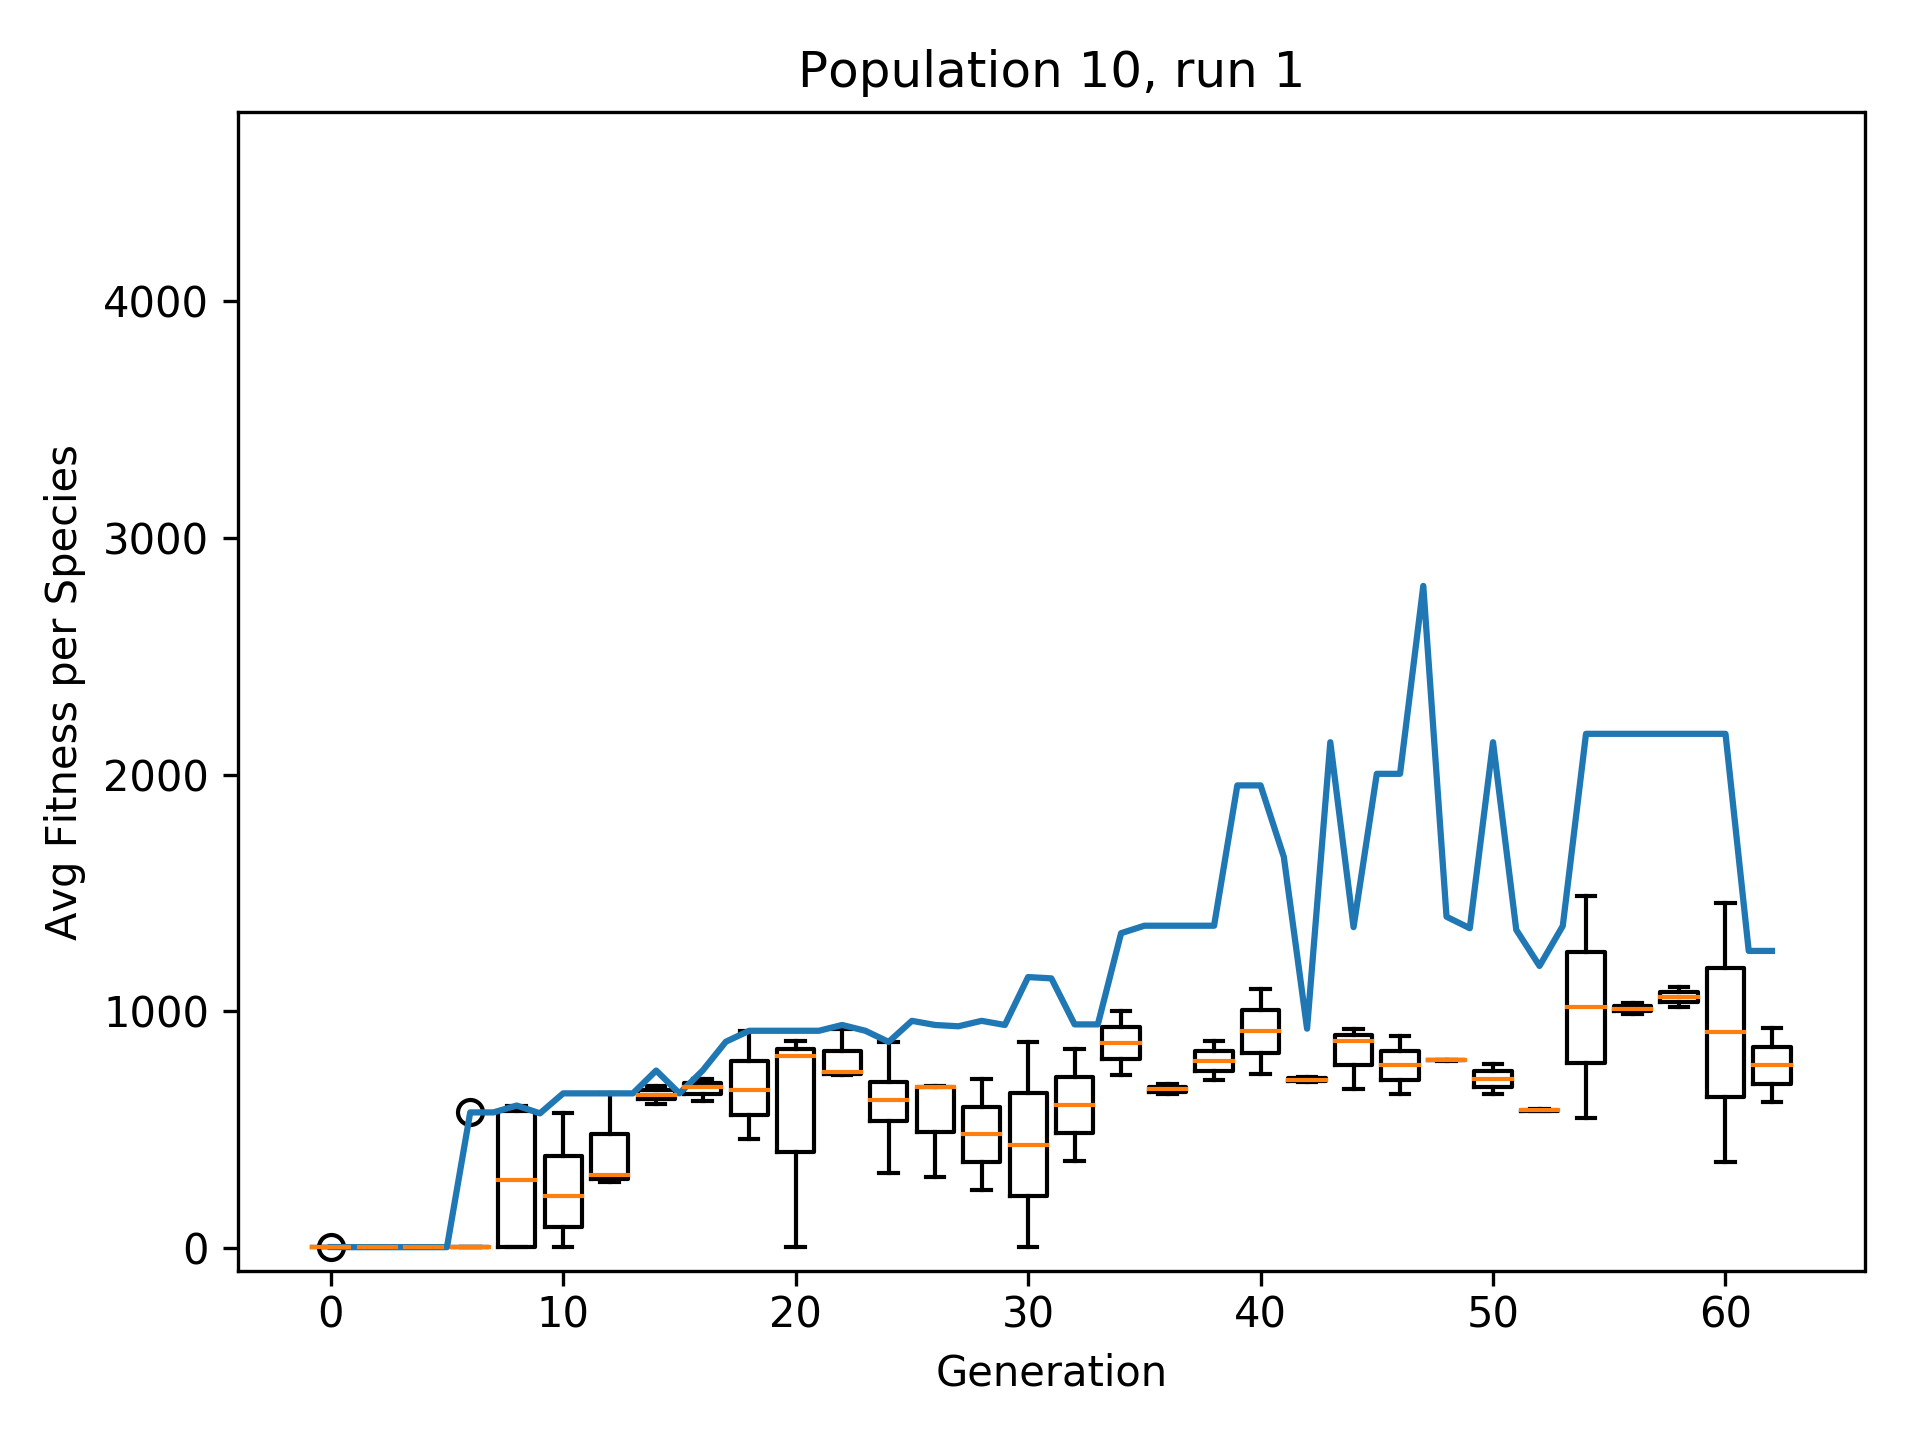
\includegraphics[width=1\textwidth]{graphics/mario/pop10_run1} % first figure itself
%				\end{minipage}\hfill
%				\begin{minipage}{0.33\textwidth}
%					\centering
%					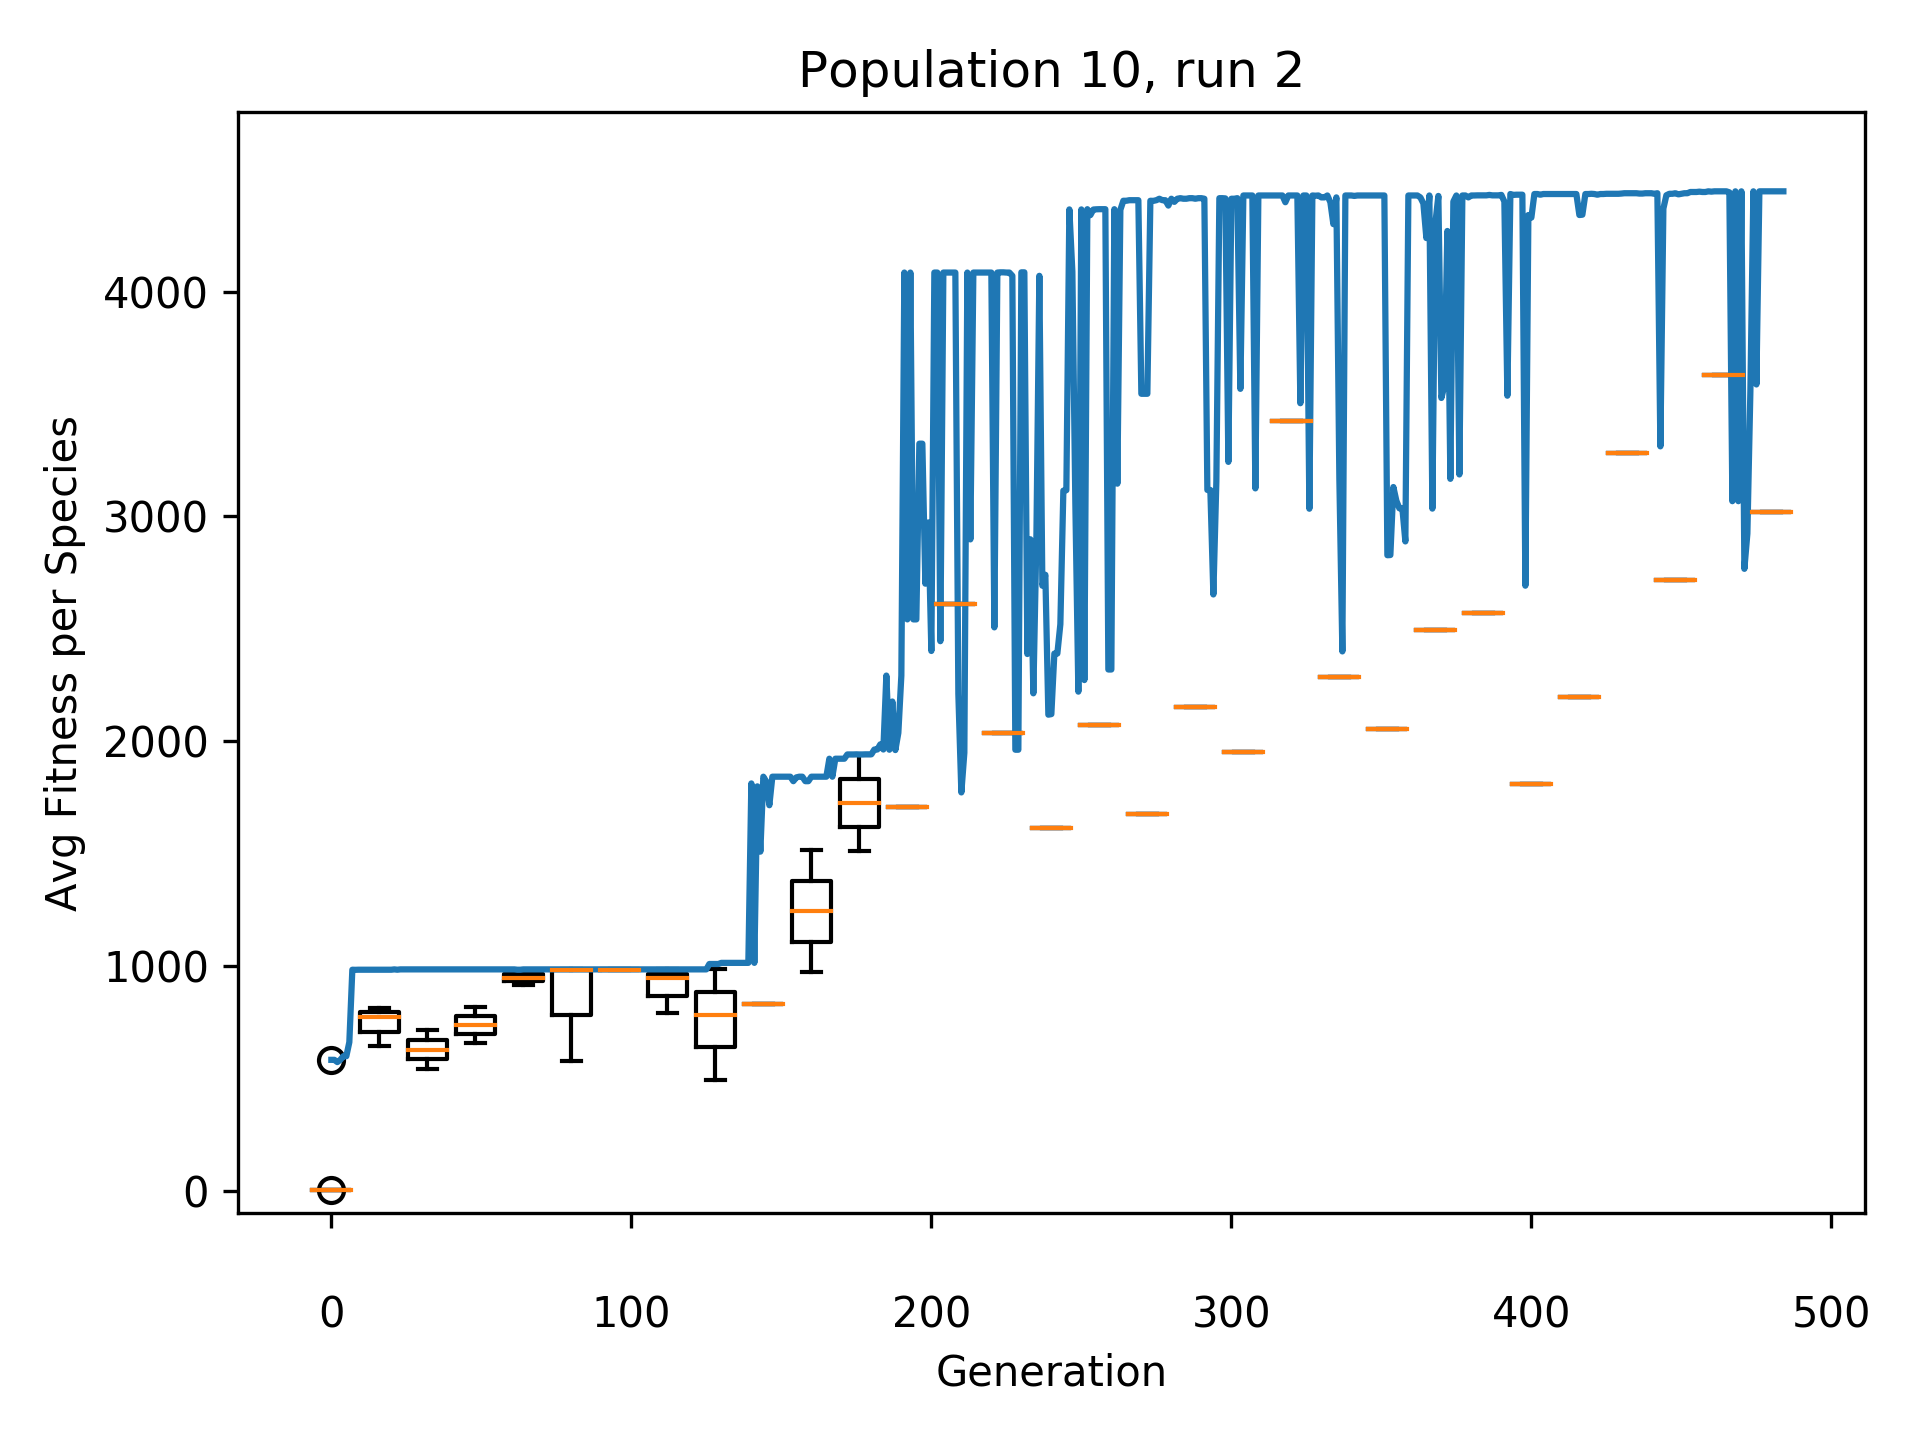
\includegraphics[width=1\textwidth]{graphics/mario/pop10_run2} % second figure itself
%				\end{minipage}
%				\begin{minipage}{0.33\textwidth}
%					\centering
%					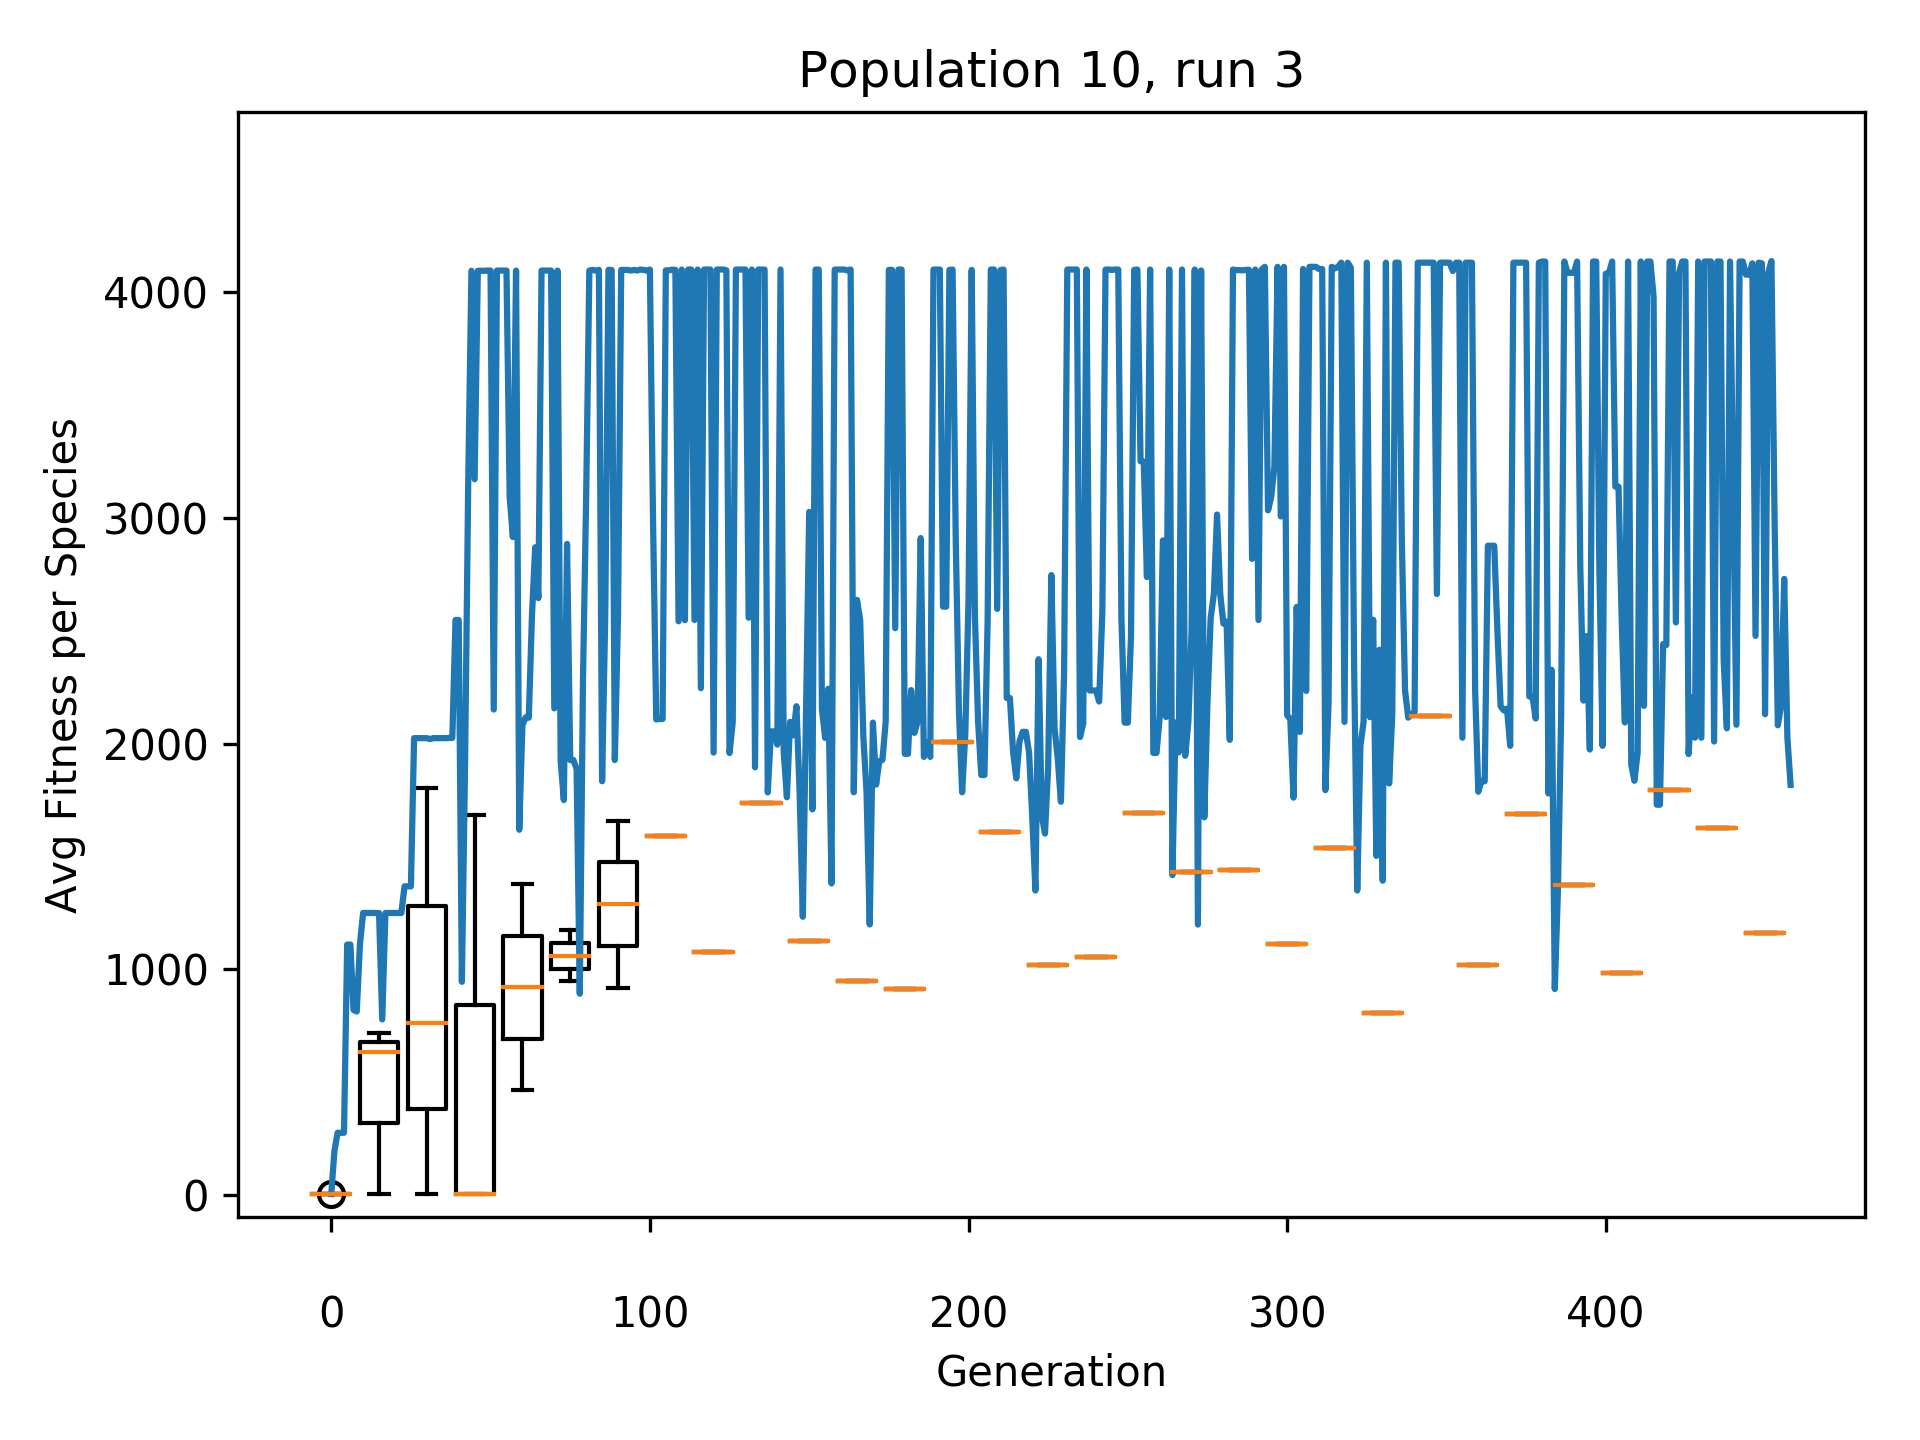
\includegraphics[width=1\textwidth]{graphics/mario/pop10_run3} % second figure itself
%				\end{minipage}
%				\caption{MarI/O Population 10}
%				\label{fig:mario10}
%			\end{figure}
			As it is visible in Figure \ref{fig:mario10} the vertical axis shows the fitness score average of the genomes within a species. The horizontal axis portrays the generations containing the species. Each generation contains up to 10 populations which is divided into species and genomes within species. This species devision was made based on the NEAT algorithm described in section \ref{sec:related:neat}. The best run of the genomes grouped by each generation is marked with a blue line. Therefore the blue line indicates the best overall run within a generation. Since the boxplot portrays the species's avarage score of each generation and the the blue line shows the best run per genome (population), the boxplot and the blue line rarely meet. Still the average population score is closer to the best run than in the next two population variants (see later in this section population 50 \ref{par:mario50} and population 250 \ref{par:mario250}). This can be calculated by taking the median of the species fitnesses and substracting that number from the best run of the genomes:
			$average\_distance = \frac{\sum\nolimits_{g_i \in generations} max(g_i.genomes) - median(g_i.species)}{|generations|}\approx1107$ whereas $g_i.genomes$ and $g_i.species$ are lists of the respective fitnesses. \\
			In the three runs on average $334.\overline{6}$ generations were created which results in a skipping of generations inside the graphics of around $11.1\overline{5}$ generations averagely between two displayed generations. Unfortunately the first run crashed after generation 60. Still, because of the long runtime of the simulation the run was kept. However, indicated by plot run 2 and 3, the population growth started after this generation. As it can be seen in the 3rd run of the figure \ref{fig:mario10}, sometimes runs over 3000 fitness score could be achieved even after the 30th generation. In run 2 the average fitness of the species tend to rise, however more and longer runs would be needed to test this hypothesis.\\
			In each generations there are up to 10 populations. \todo{(up to because of neat implementation check neat implementation}
			In the first generation (Gen 0) no mating was done, so in the first generation there where 10 species spawned with one genome each. In the 10th Generation on average only $4.\overline{3}$ species where left. After generation 50 maximum 3 species where left in all runs and after generation 190 in run 2 and after generation 91 in run 3, respectively, only 1 species was left for mating. The mating results into the corssover of species.\\
			All runs except plot run 1 reached the goal (the end of the level) multiple times which can be seen by the fitnesscore being over 4000. However plot run 3 reached the goal the earliest with runs over 4096 starting from generation 44. Still there was the most overall regress made in plot run 3. This can be calculated by adding the differences between the best runs of each generation if the difference was negative: $average\_regress = \frac{\sum\nolimits_{g_i \in generations} min(max(g_i.genomes) - max(g_{i-1}.genomes), 0)}{|generations|}\approx-348$ again whereas $g_i.genomes$ is a list of the fitnesses of each genome inside the generation. The regress of plot-run 1 was $-88.27$ approximately and of plot-run 2 was around $-109.98$.\\
			In plot run 1 the $average\_fitness\_increase =  \frac{\sum\nolimits_{g_i \in generations} max(g_i.genomes) - max(g_{i-1}.genomes)}{|generations|}\approx19.87$ was the biggest of the three runs since run 1 ended early and run 3 had many drawbacks. The average fitness increase of run 2 was around $7.97$ and of run 3 was only $3.95$ approximately. Since it is only slightly possible to extend the maximum score above the score of 4000 and run 1 has never reached this ranking, run 1 pointed out to have the best score increase per round. Every successful round, whereas Mario reached the goal will only minimize the fitness increase when averaged with the generation count. In another words, for an infinitely large amount of generations the $average\_fitness\_increase$ is expected to converge to $0$ since the game has and end-state in contrast to the game Flappy Bird, as it can be seen in section \ref{sec:analysis:flappy}. In mathematical terms: $\lim\limits_{n \to \infty} average\_fitness\_increase(n) = 0$, whereas the $average\_fitness\_increase(n)$ is defined as the average fitness increase of a set of n generations.
			
			\begin{enumerate}
				\item there are up to 10 populations in each generation (up to because of neat implementation \todo{check neat implementation})
				\item Differences similarities between runs
			\end{enumerate}
		
		\paragraph{Population 50 / Generation 100}
			\label{par:mario50}
			\begin{figure}[h]
				\centering
				\begin{minipage}{0.33\textwidth}
					\centering
					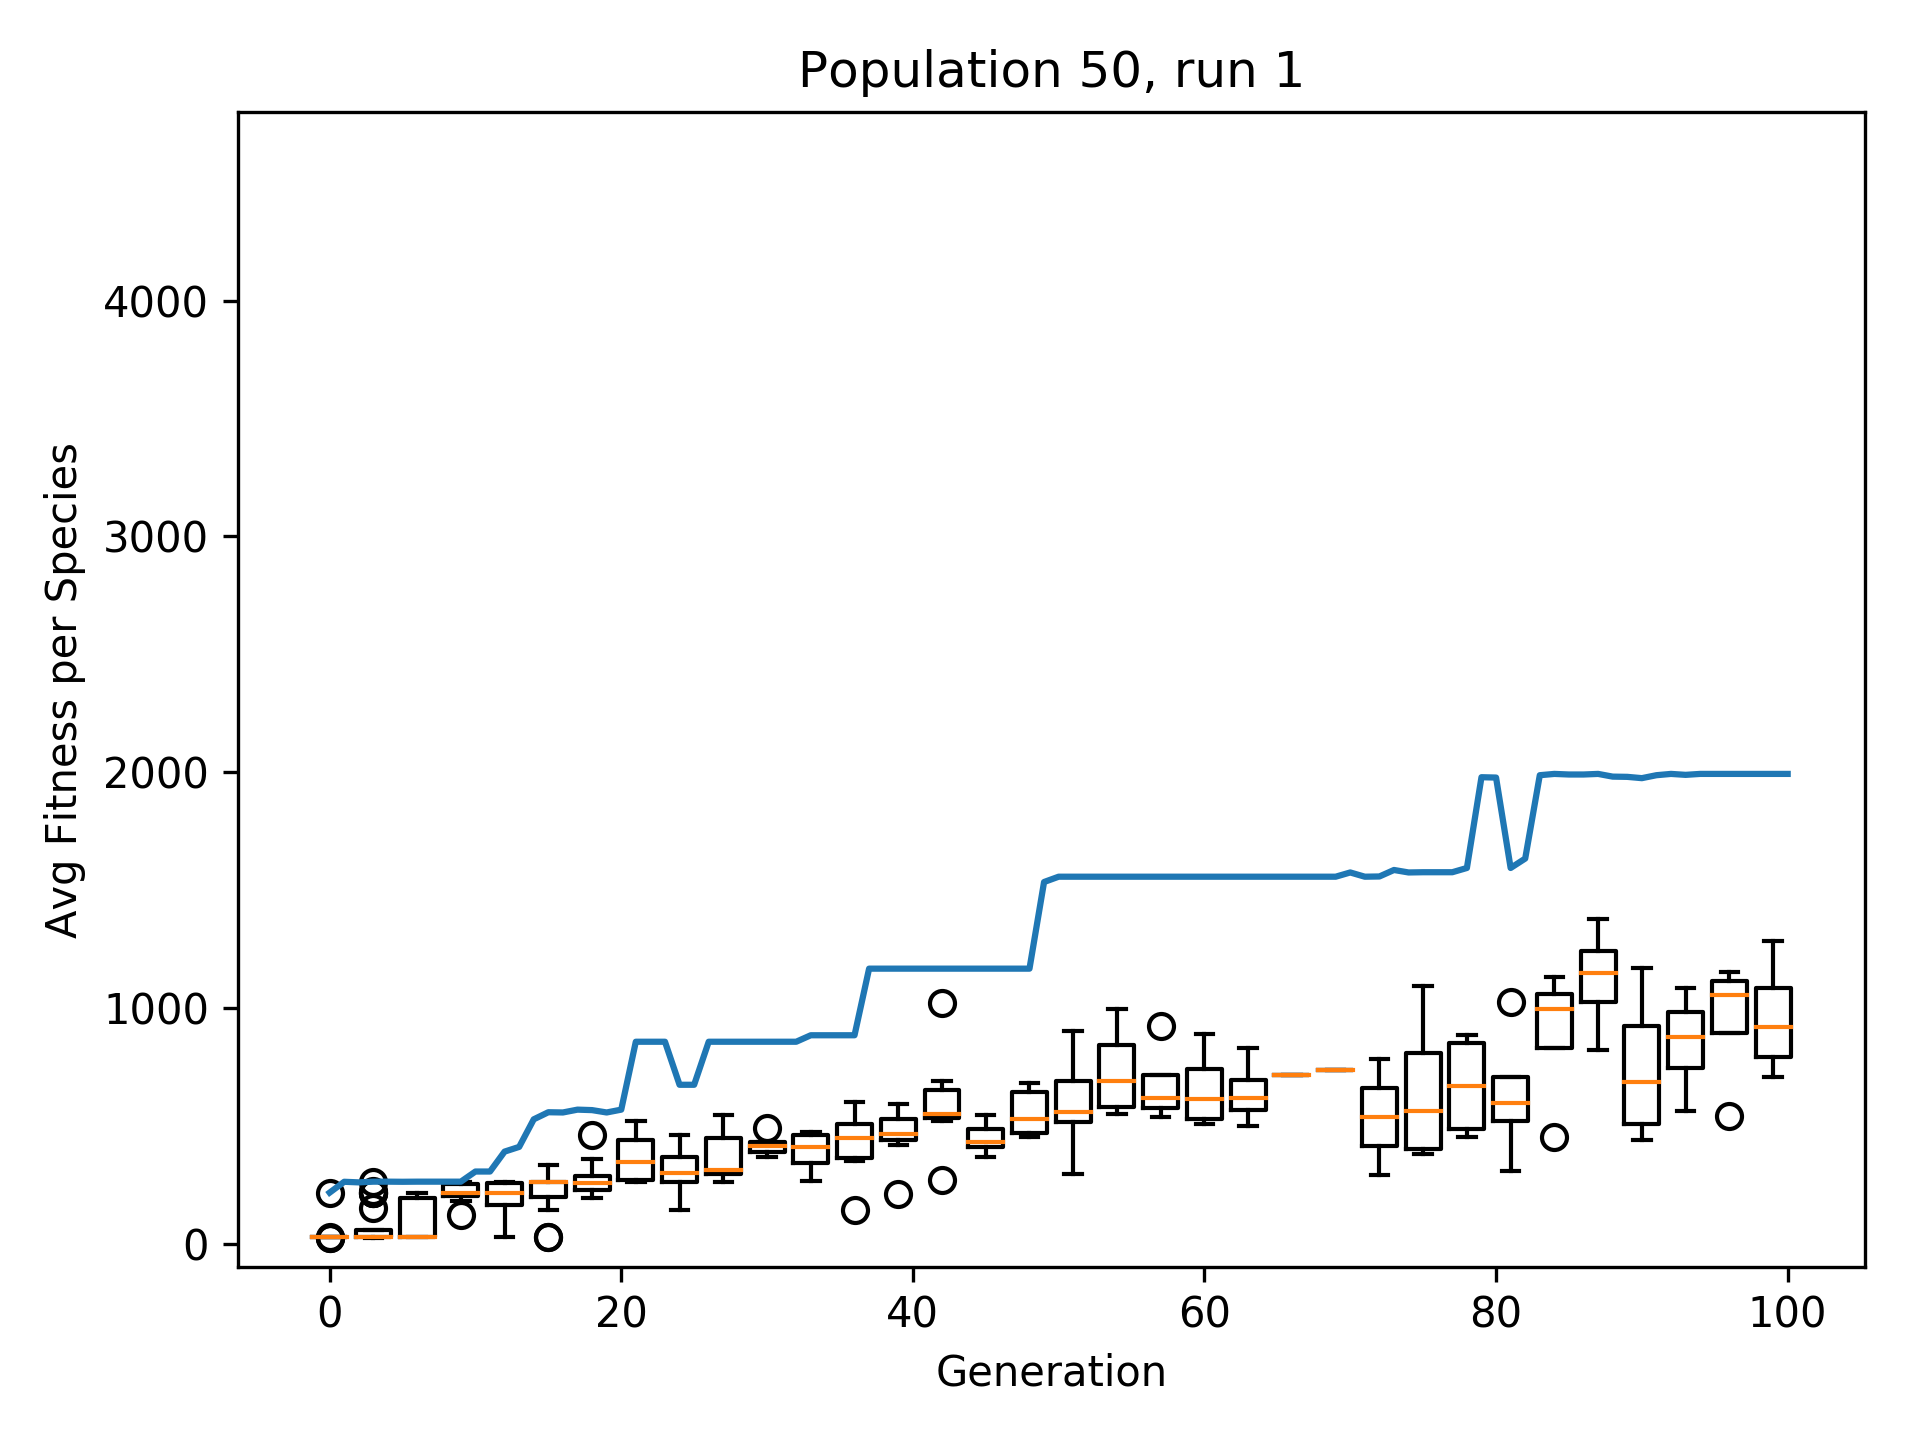
\includegraphics[width=1\textwidth]{graphics/mario/pop50_run1} % first figure itself
				\end{minipage}\hfill
				\begin{minipage}{0.33\textwidth}
					\centering
					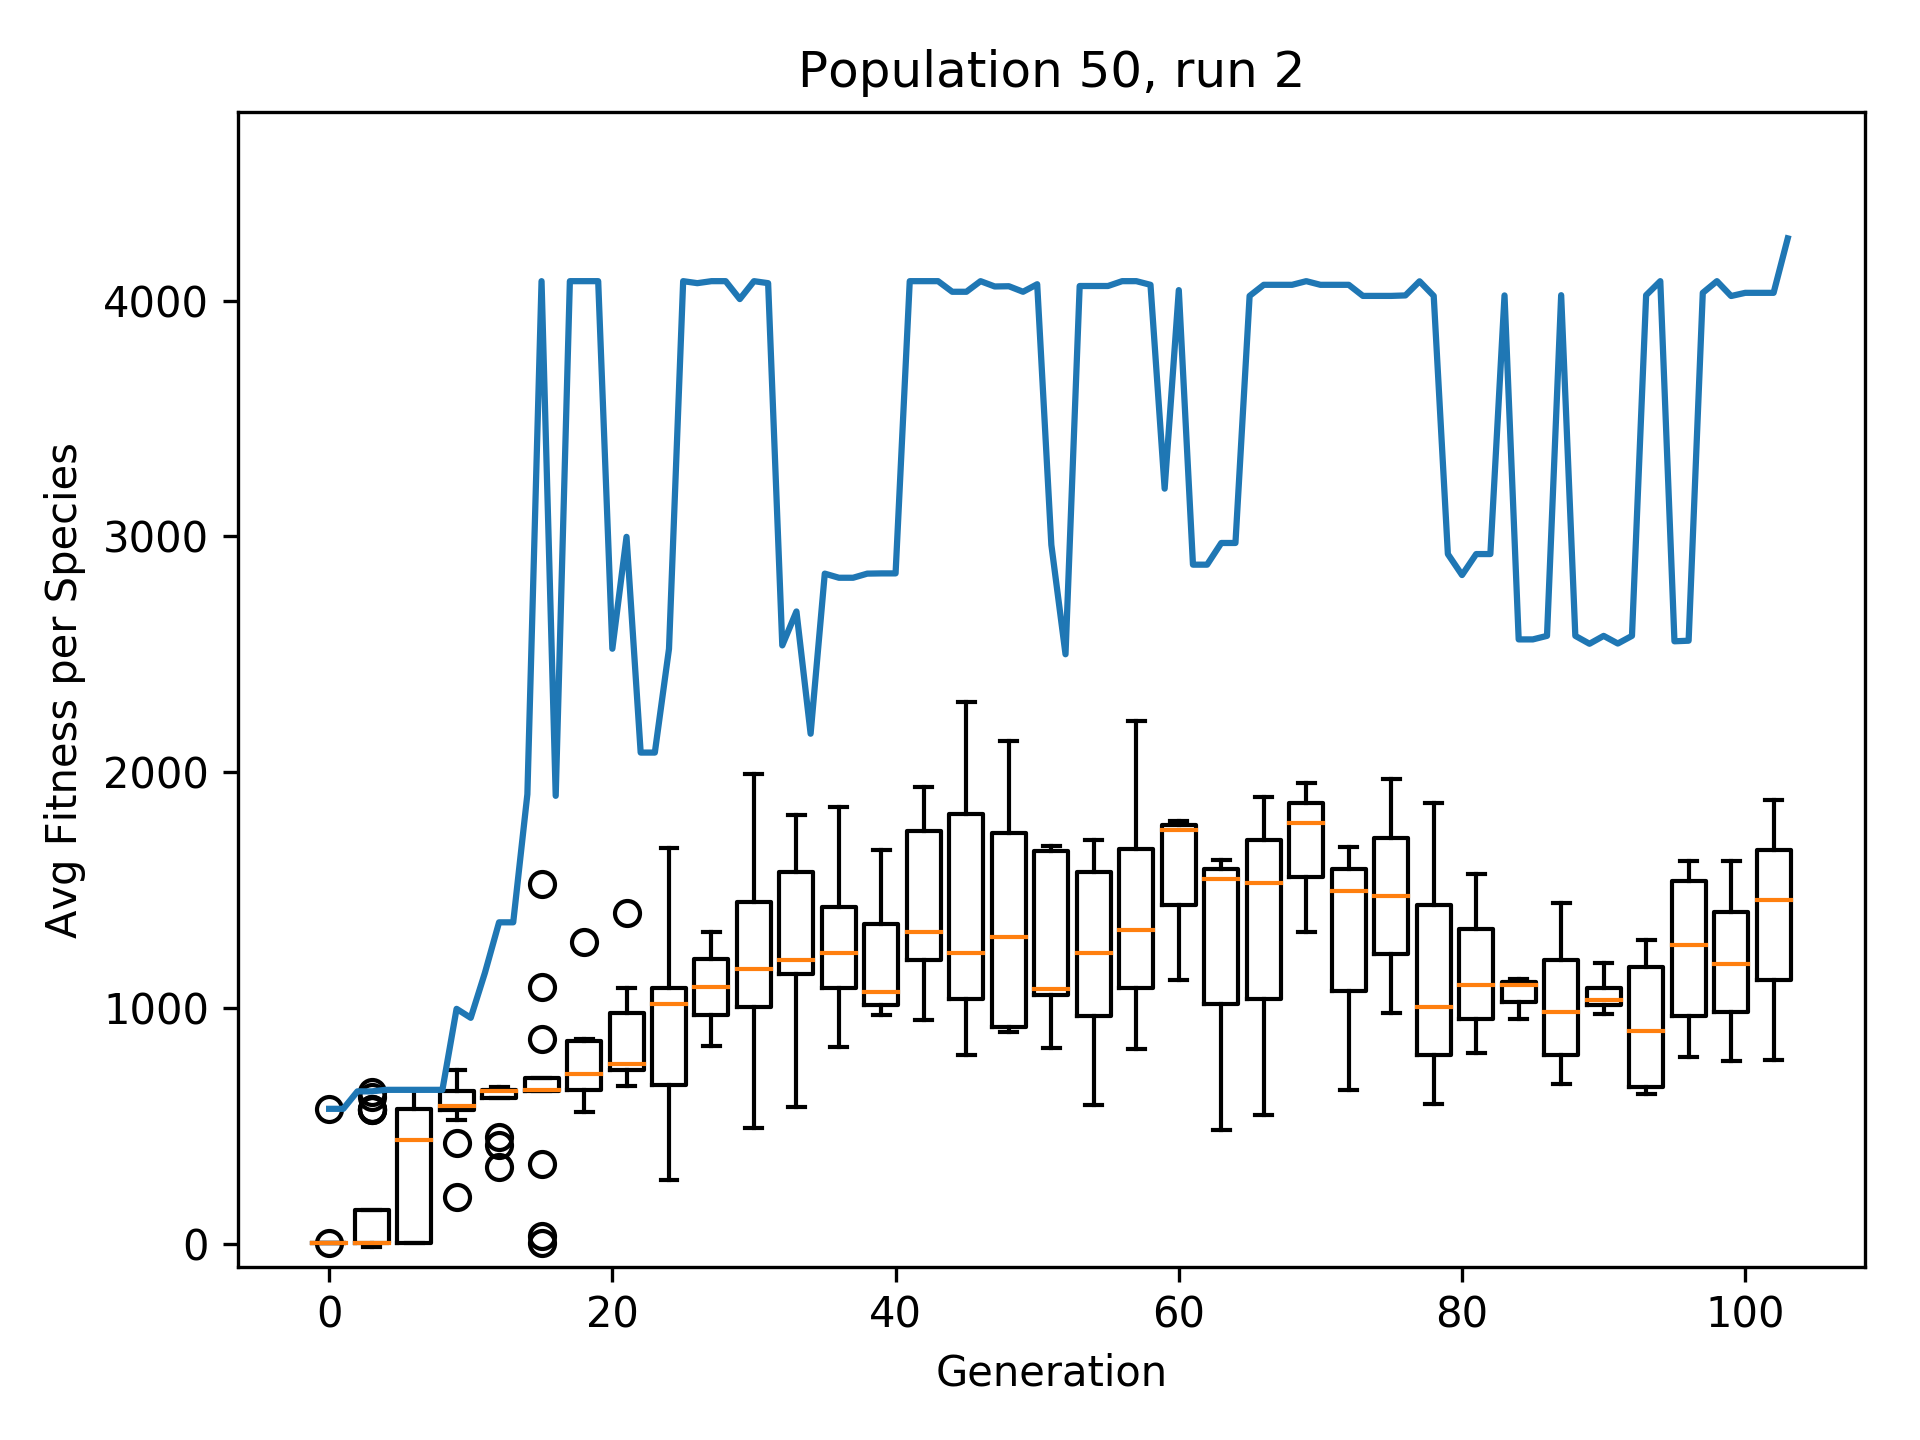
\includegraphics[width=1\textwidth]{graphics/mario/pop50_run2} % second figure itself
				\end{minipage}
				\begin{minipage}{0.33\textwidth}
					\centering
					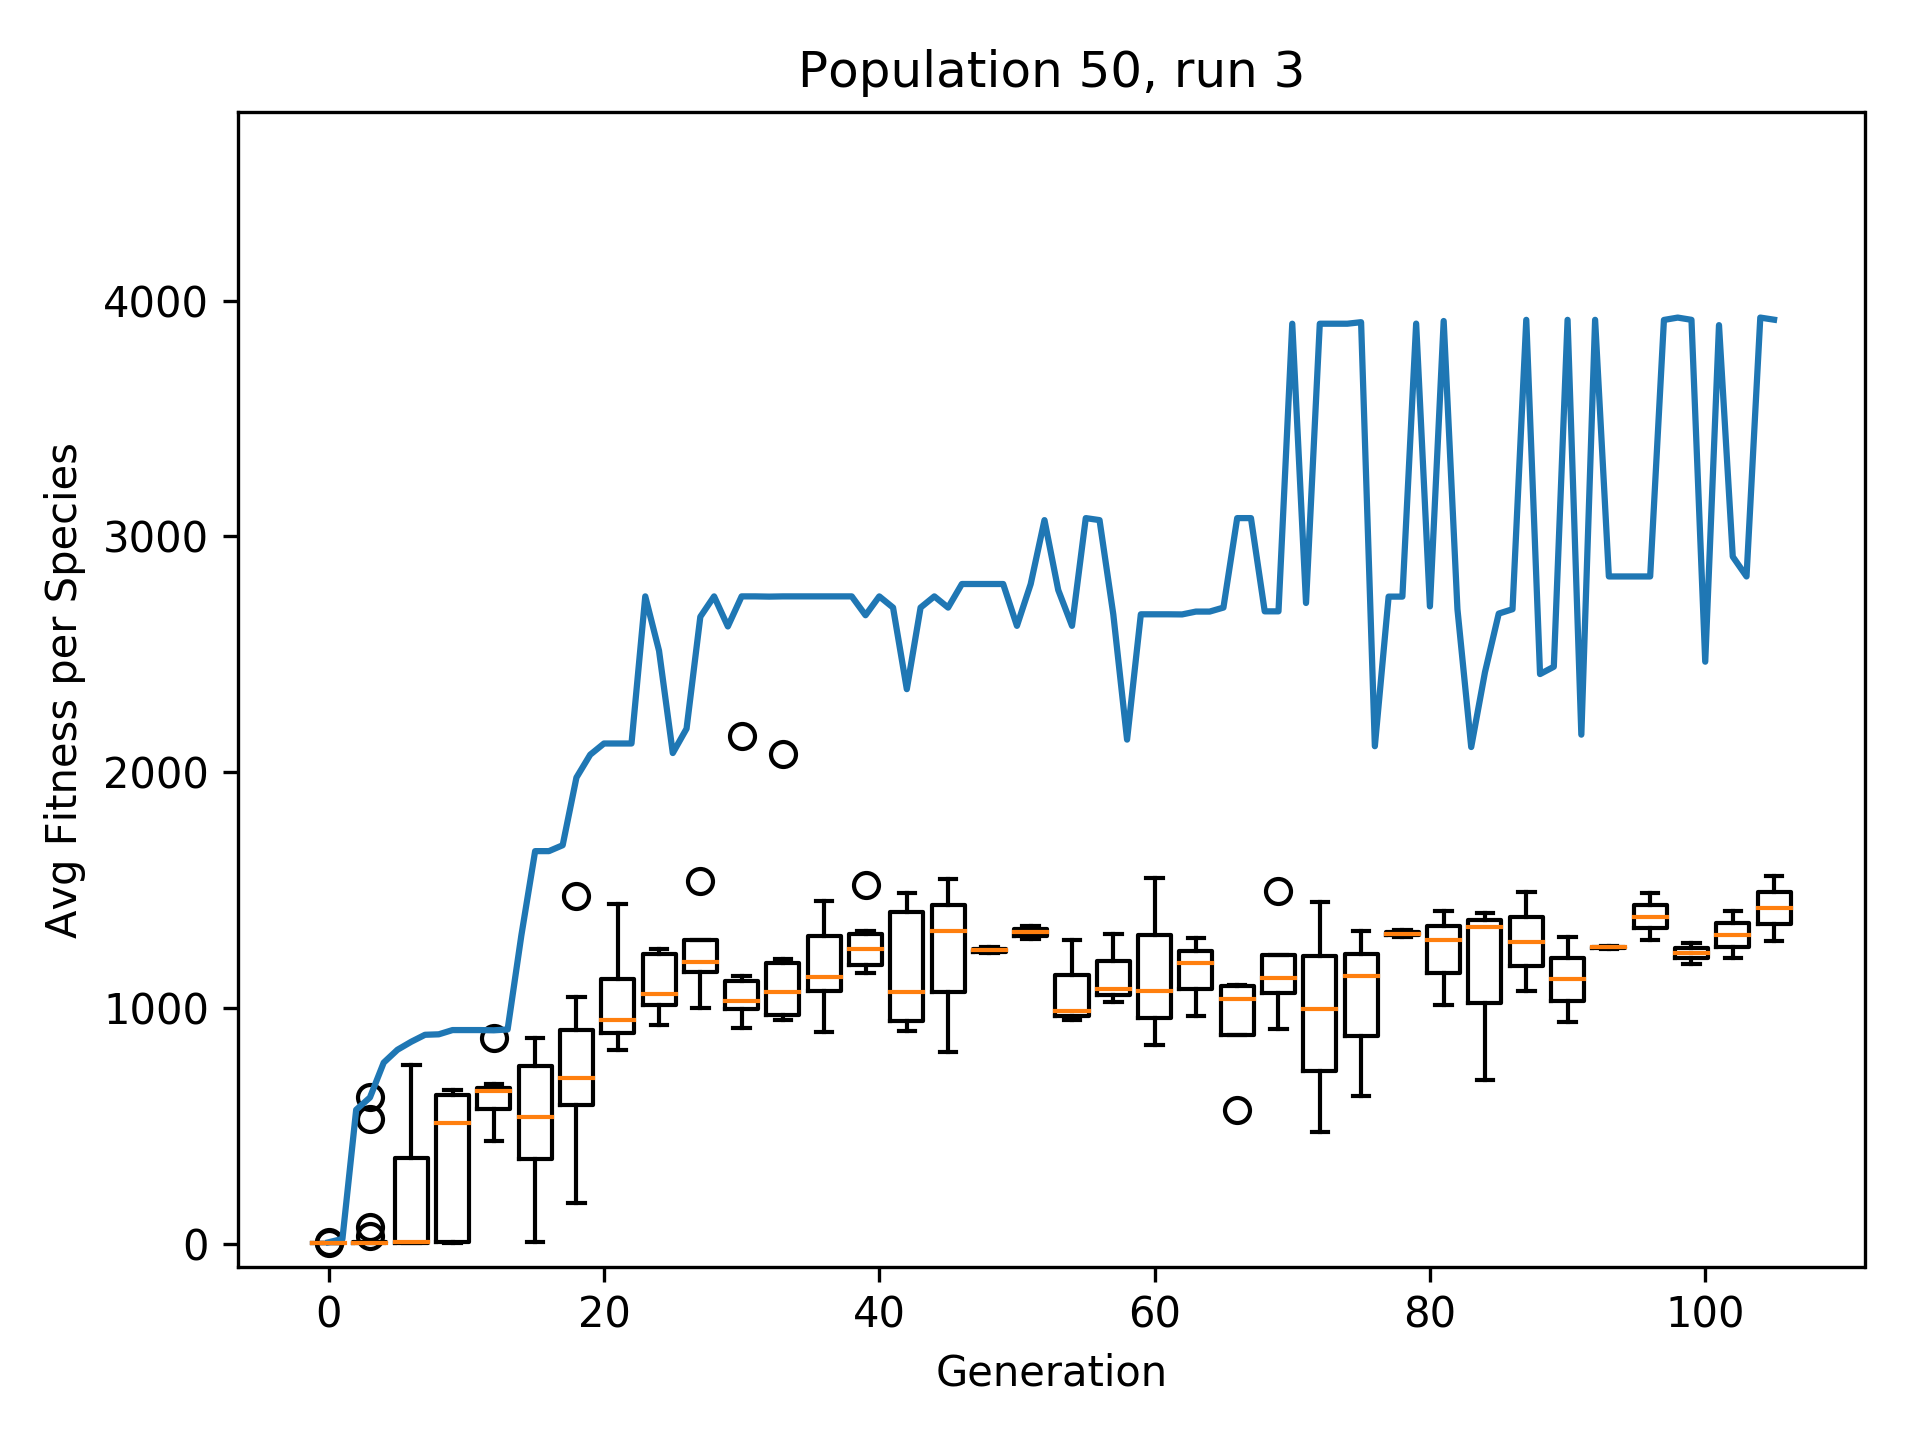
\includegraphics[width=1\textwidth]{graphics/mario/pop50_run3} % second figure itself
				\end{minipage}
				\caption{MarI/O Population 50}
				\label{fig:mario50}
			\end{figure}
			In this setup the population count is up to 50, again distributed into species and genomes within species according to the MarI/O NEAT implementation. The $average\_distance$  between the median of the species of each generation to the best genome run of this generation is bigger than that of the simulation with it's initial population size of 10 but it is smaller than in the last case. The $average\_distance$ was calculated as described in the previous simulation (population 10 \ref{par:mario10}) and the value is approximately $1406$.\\
			In this simulations the runs where executed until there where over 100 generations (101 generations in run 1, 104 in run 2 and 106 in run 3). This results in an average skipping of 3.456 generations between the display of two generations.\\
			In generation 0 there where 50 species spawned, again, with one genome each. In the 10th generation there where 15 species left on average. At the end of generation 100 on average $3.\overline{3}$ species where left from the initial 50 generations.\\
			Interestingly the plot run 1 couldn't learn to reach the goal. From this data it is not trivial to predict if the breakthrough would have started within the next 50 generations or if this run would have stayed low in it's fitness score, since there are no clear patterns to find in the graphical representation of these runs. In order to answer on this question more profoundly, further and longer runs have to be made and the big jumps between the fitness scores of each neighbour generation would have to be analysed.\\
			Plot run 2 and 3 had more luck in reaching the end, however run 3 had more stability in it's high score results between generations. Still after generation 70 plot run 3 also shows stronger differences between it's generation's heigh scores. Nevertheless, plot-run 2 reached the goal the earliest. The first time run 2 acheived a fitness-score over 4000 was in generation 15 (it reached a score of $4082.5$), whereas plot-run 3 reached a maximum score of $3928$ in generation 98. Still run 3 reached to goal with a score of $3902$ the first time in generation 70. The 3rd plot-run has the highest $average\_fitness\_increase\approx36.92$ of the three runs. Plot-run 1 has an $average\_fitness\_increase$ of $17.58$ approximately and plot-run 2 of $35.5$ precisely.\\
		
		
		\paragraph{Population 250 / Generation 30}
			\label{par:mario250}
			\begin{figure}[h]
				\centering
				\begin{minipage}{0.33\textwidth}
					\centering
					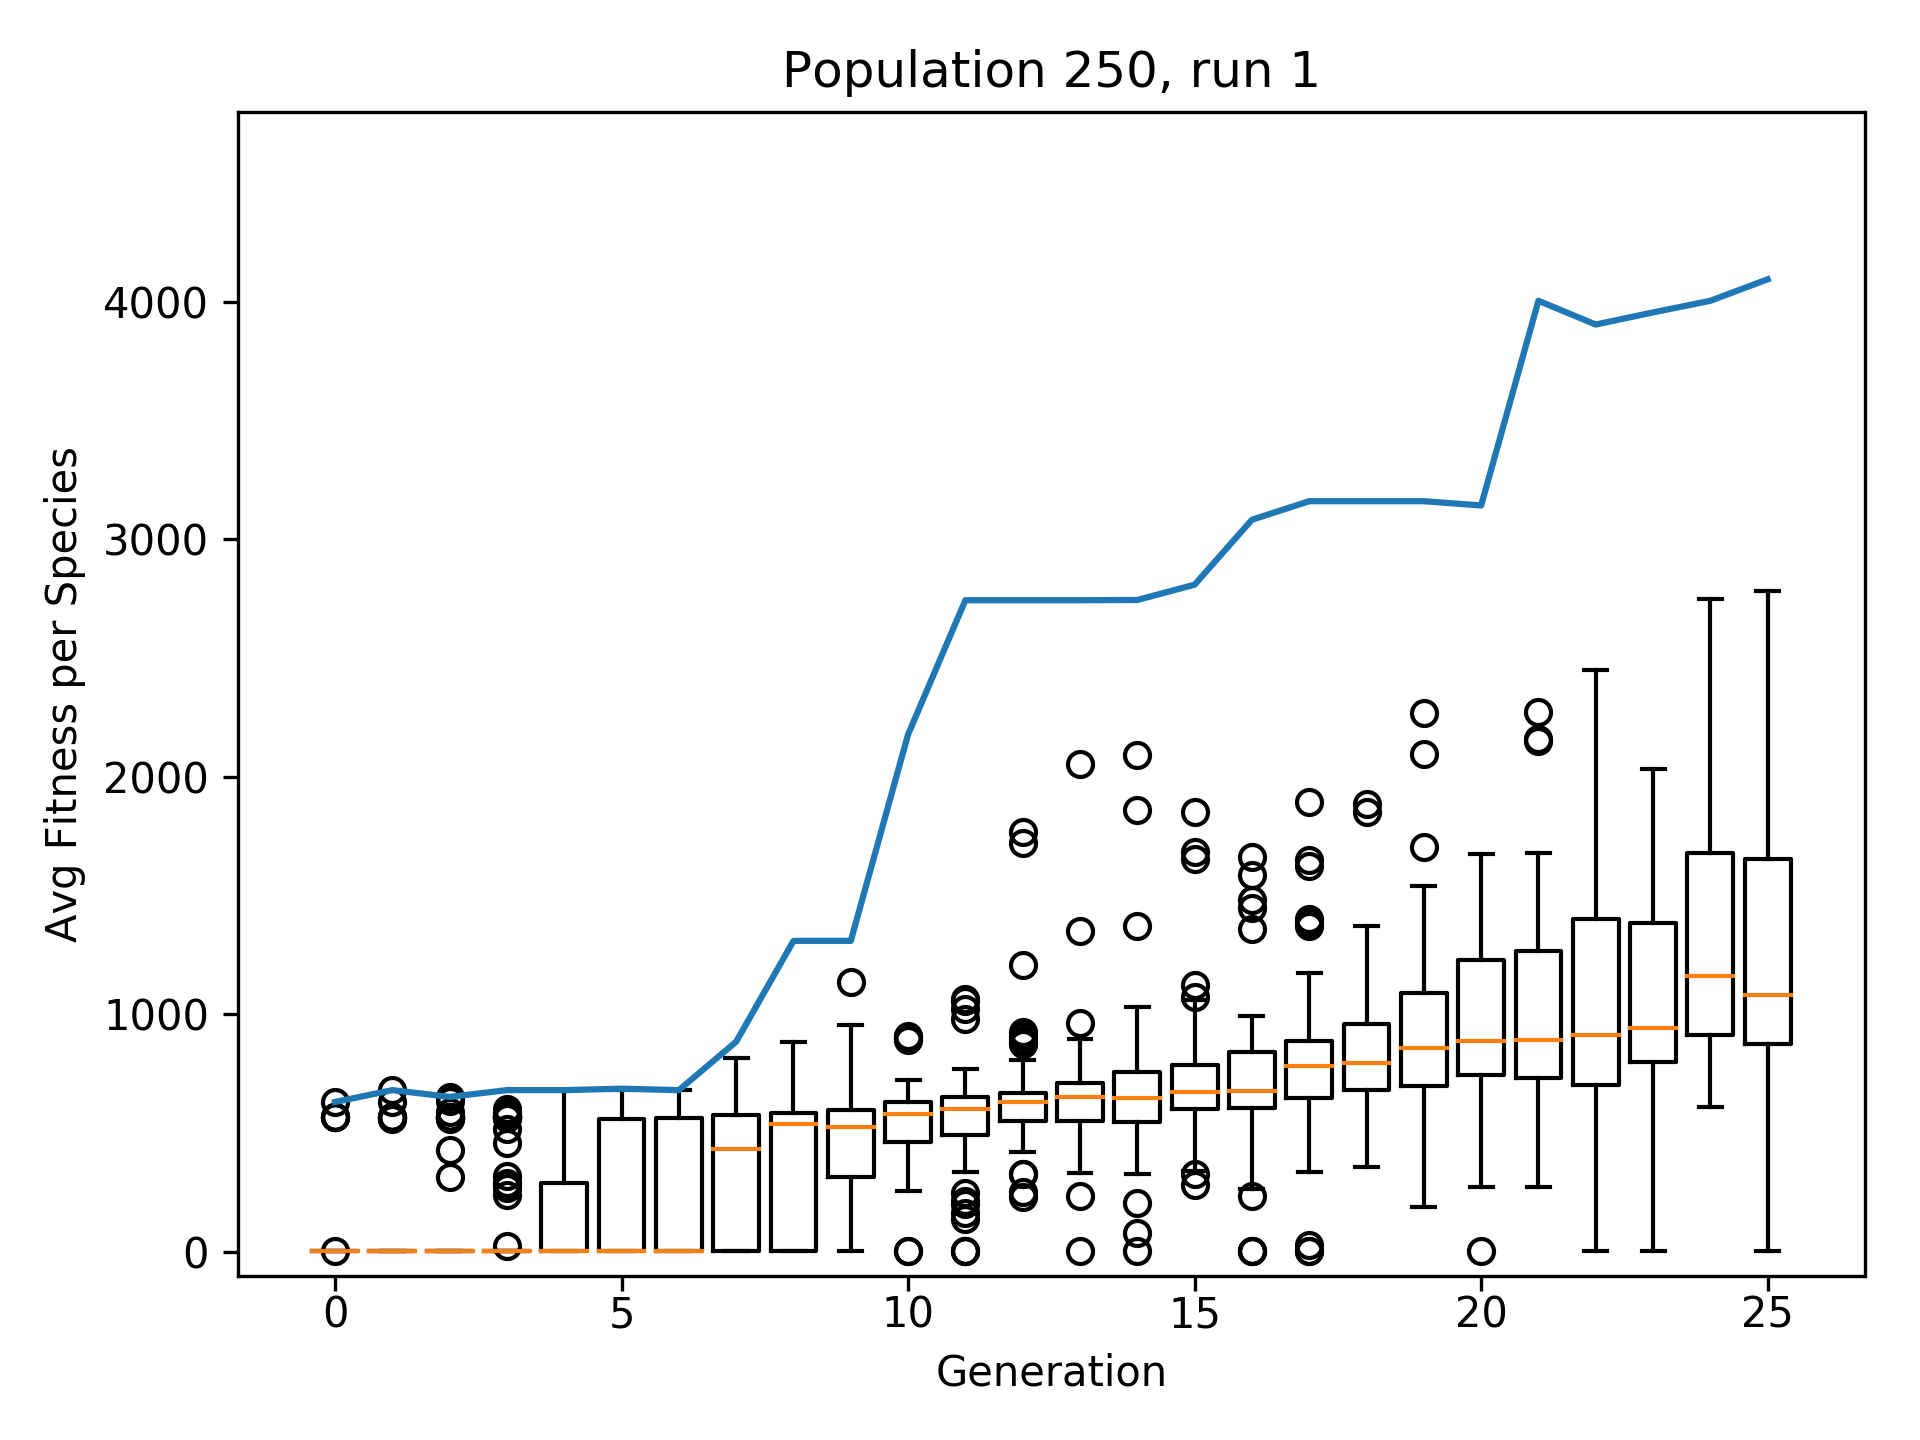
\includegraphics[width=1\textwidth]{graphics/mario/pop250_run1} % first figure itself
				\end{minipage}\hfill
				\begin{minipage}{0.33\textwidth}
					\centering
					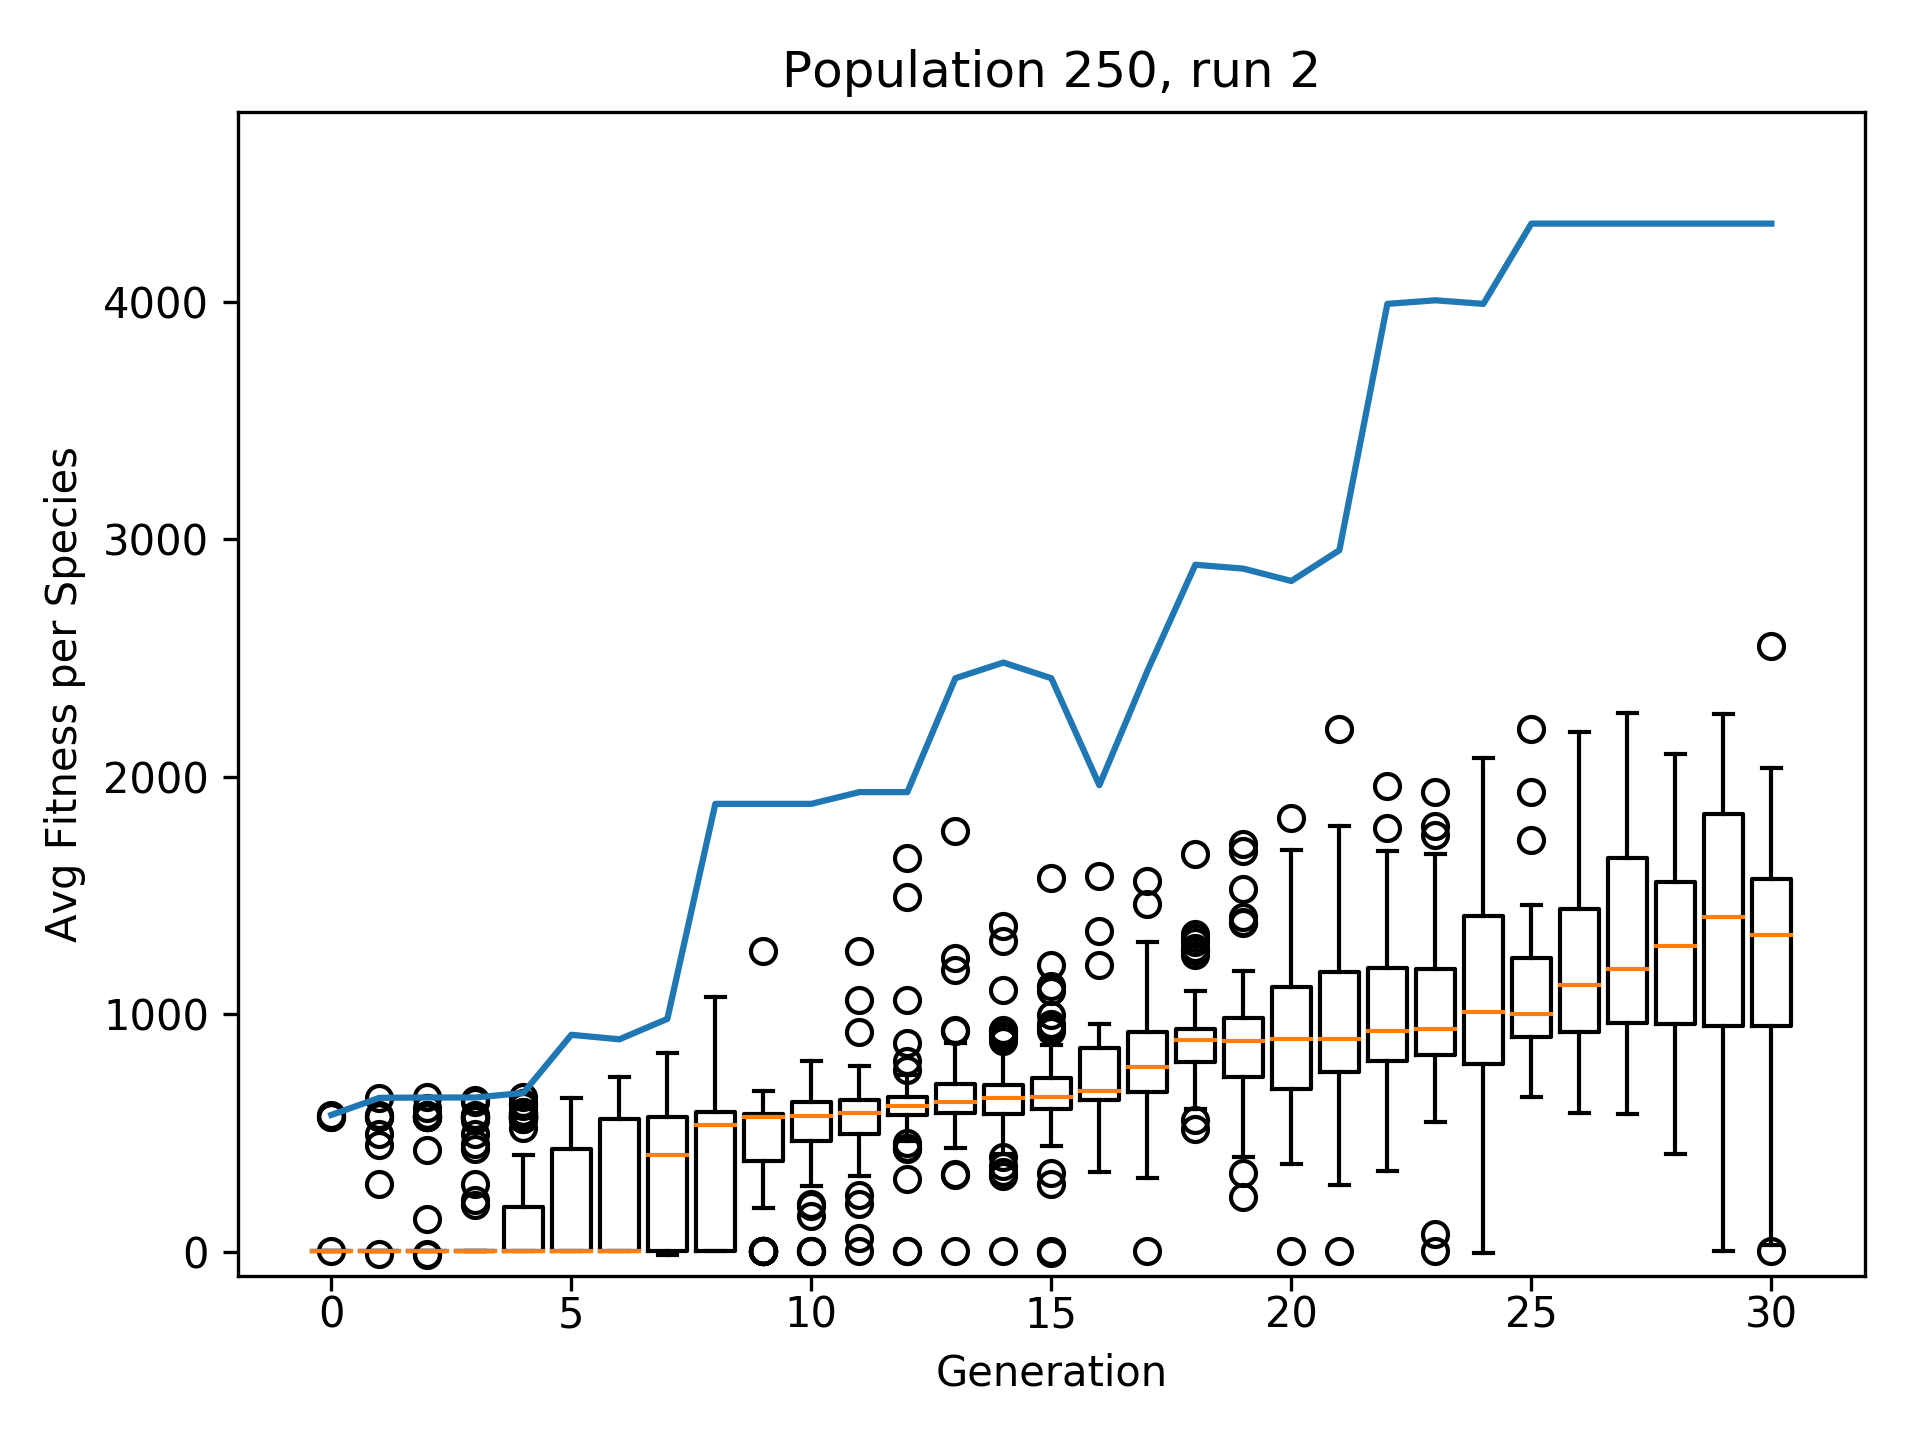
\includegraphics[width=1\textwidth]{graphics/mario/pop250_run2} % second figure itself
				\end{minipage}
				\begin{minipage}{0.33\textwidth}
					\centering
					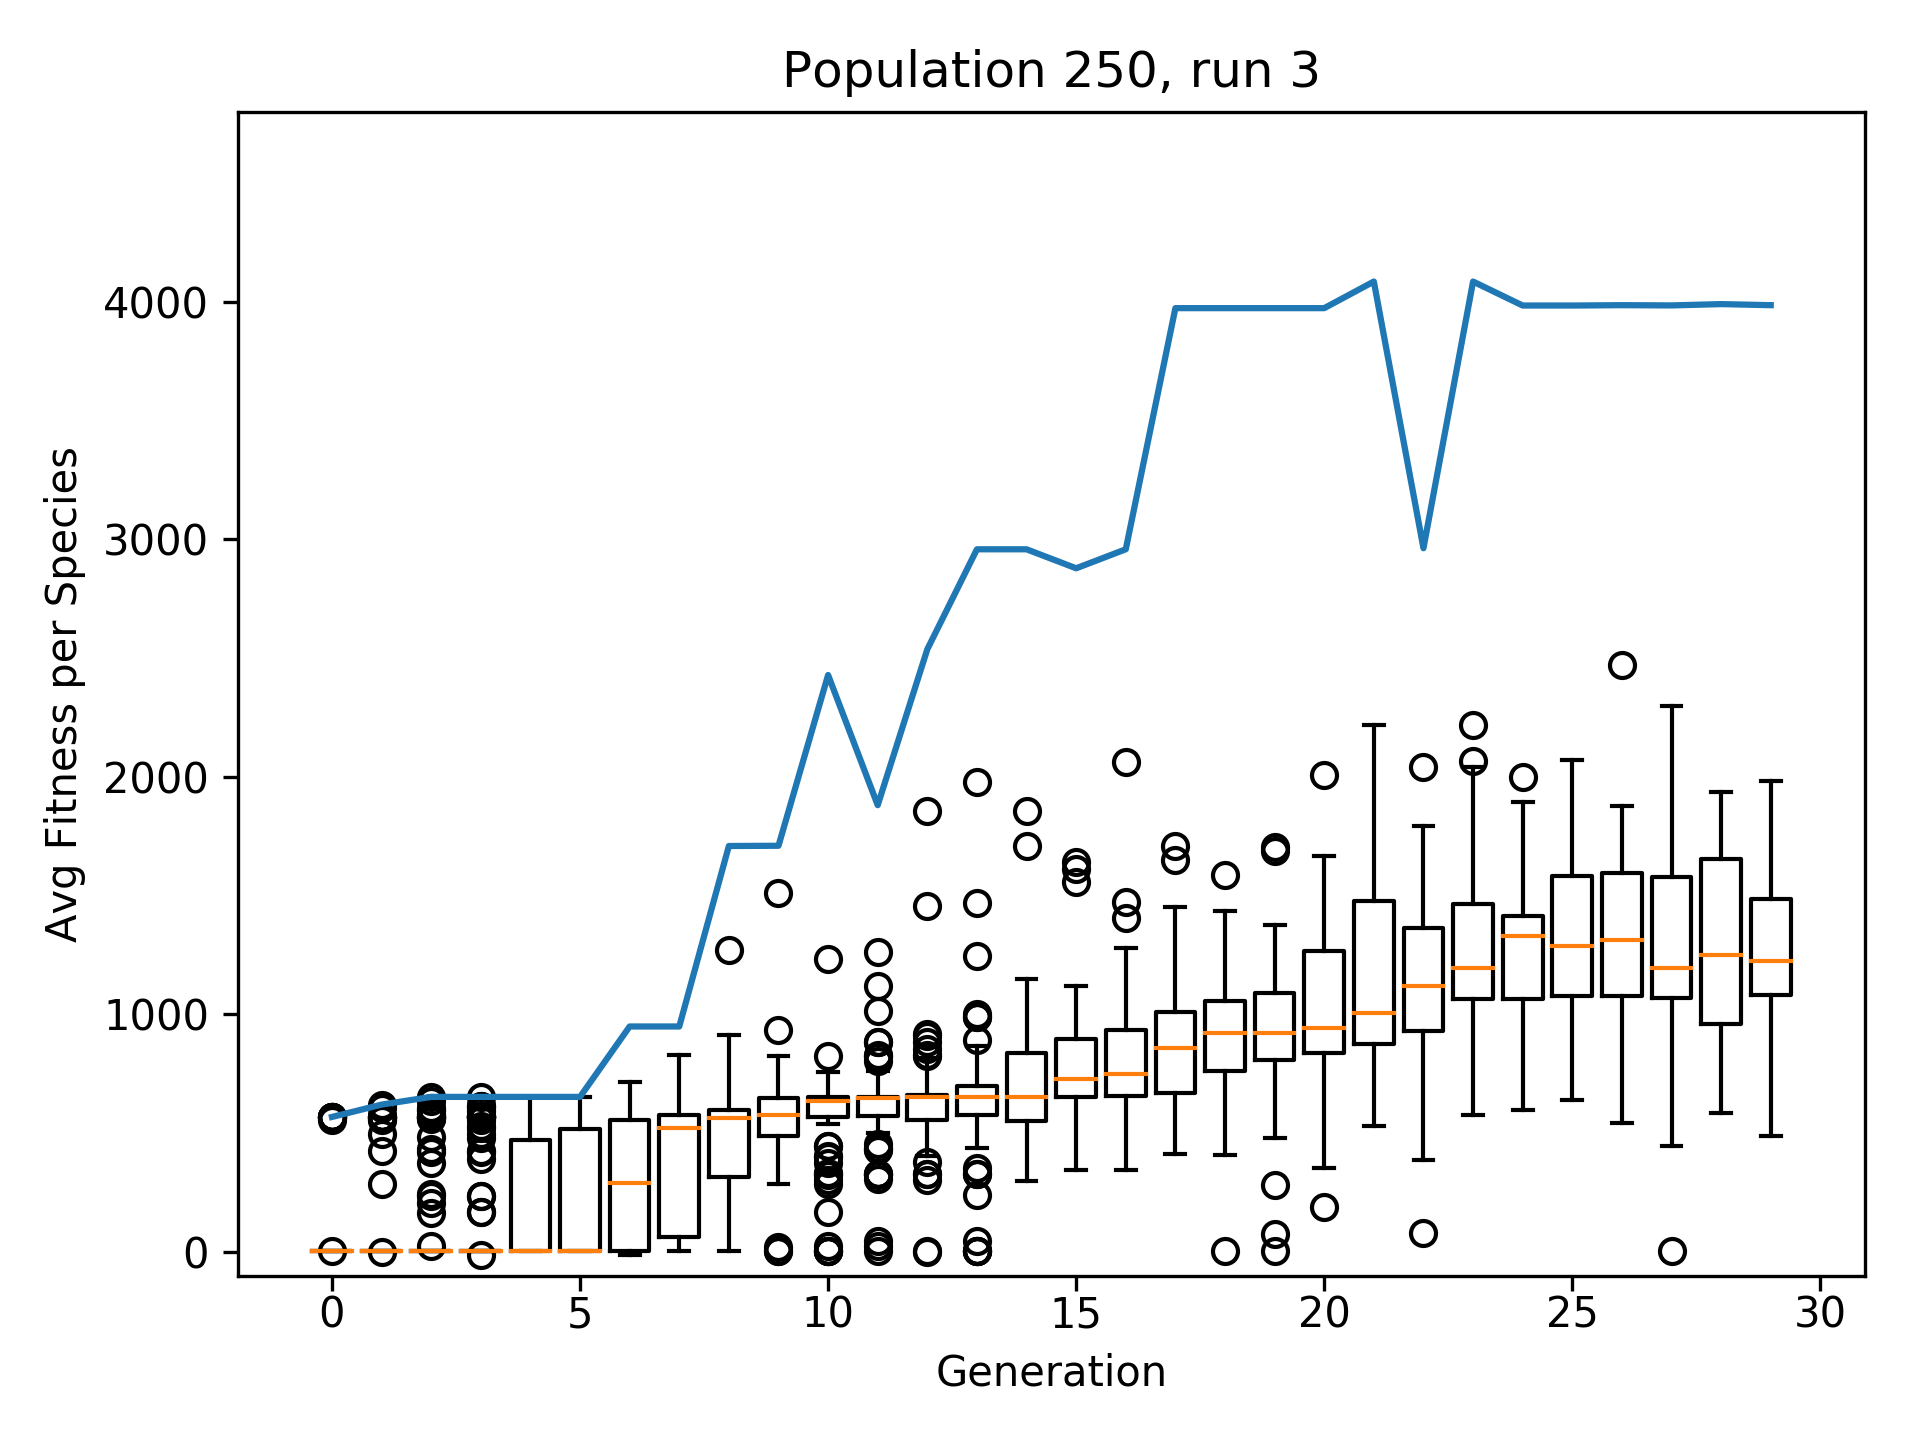
\includegraphics[width=1\textwidth]{graphics/mario/pop250_run3} % second figure itself
				\end{minipage}
				\caption{MarI/O Population 250}
				\label{fig:mario250}
			\end{figure}
			In figure \ref{fig:mario250} the population size is up to 250 in generation 0. In the first generation (Gen 0) 250 species are born with one genome each. The $average\_distance$ for this plot-runs is the biggest with approximately $1827$ when compared to the plot-runs with an initial population size of 10 and 50. In this plots no generations had to be skipped in order to portray a descriptive graph since the maximum generation count is 30 in run 2 (25 generations in run 1 and 29 generations in run 3).\\
			Already in the 6th generation, on average only 94.8 species where left. At the end of generation 25 there where 31 species left on average. \\
			Compared to the other two population classes there are at least 7 times more species left at the end of the simulations which results in longer whiskers of the boxplot.The wiskers even contains bad starts with fitness-scores lower than 100 in plot-run 1 and 2. Interestingly the best runs are always exceptions after generation 6 (in plot-run 1 and 2 even earlier). \\
			Further it is to mention that the plots are rather uniform compared to the plots of population 10 and 50. Therefore the $average\_fitness\_increase$ has similar values with a low variance which are $133.25$ for generation 1, around $121.08$ for generation 2 and $113.95$ for generation 3. The $average\_regress$ is the lowest in run 1 with $-5.87$ approximately. This is because the maximum value of the succeeding generation is smaller then the previous generation in only 4 cases. The other two plot-runs have an $average\_regress$ of approximately $-19.97$ in run 2 and $-61.92$ in run 3. All of the runs reached the end of the level even thought run 3 reached the end at generation 17, whereas plot-run 1 reached the end at generation 23 and plot-run 2 at generation 22.	
	
	% FLAPPY BIRD ###############################################################
	
	\section{Machine Learning Flappy Bird}
		\label{sec:analysis:flappy}
		\todo{change this title}
		
		\begin{figure}[h]
			\centering
			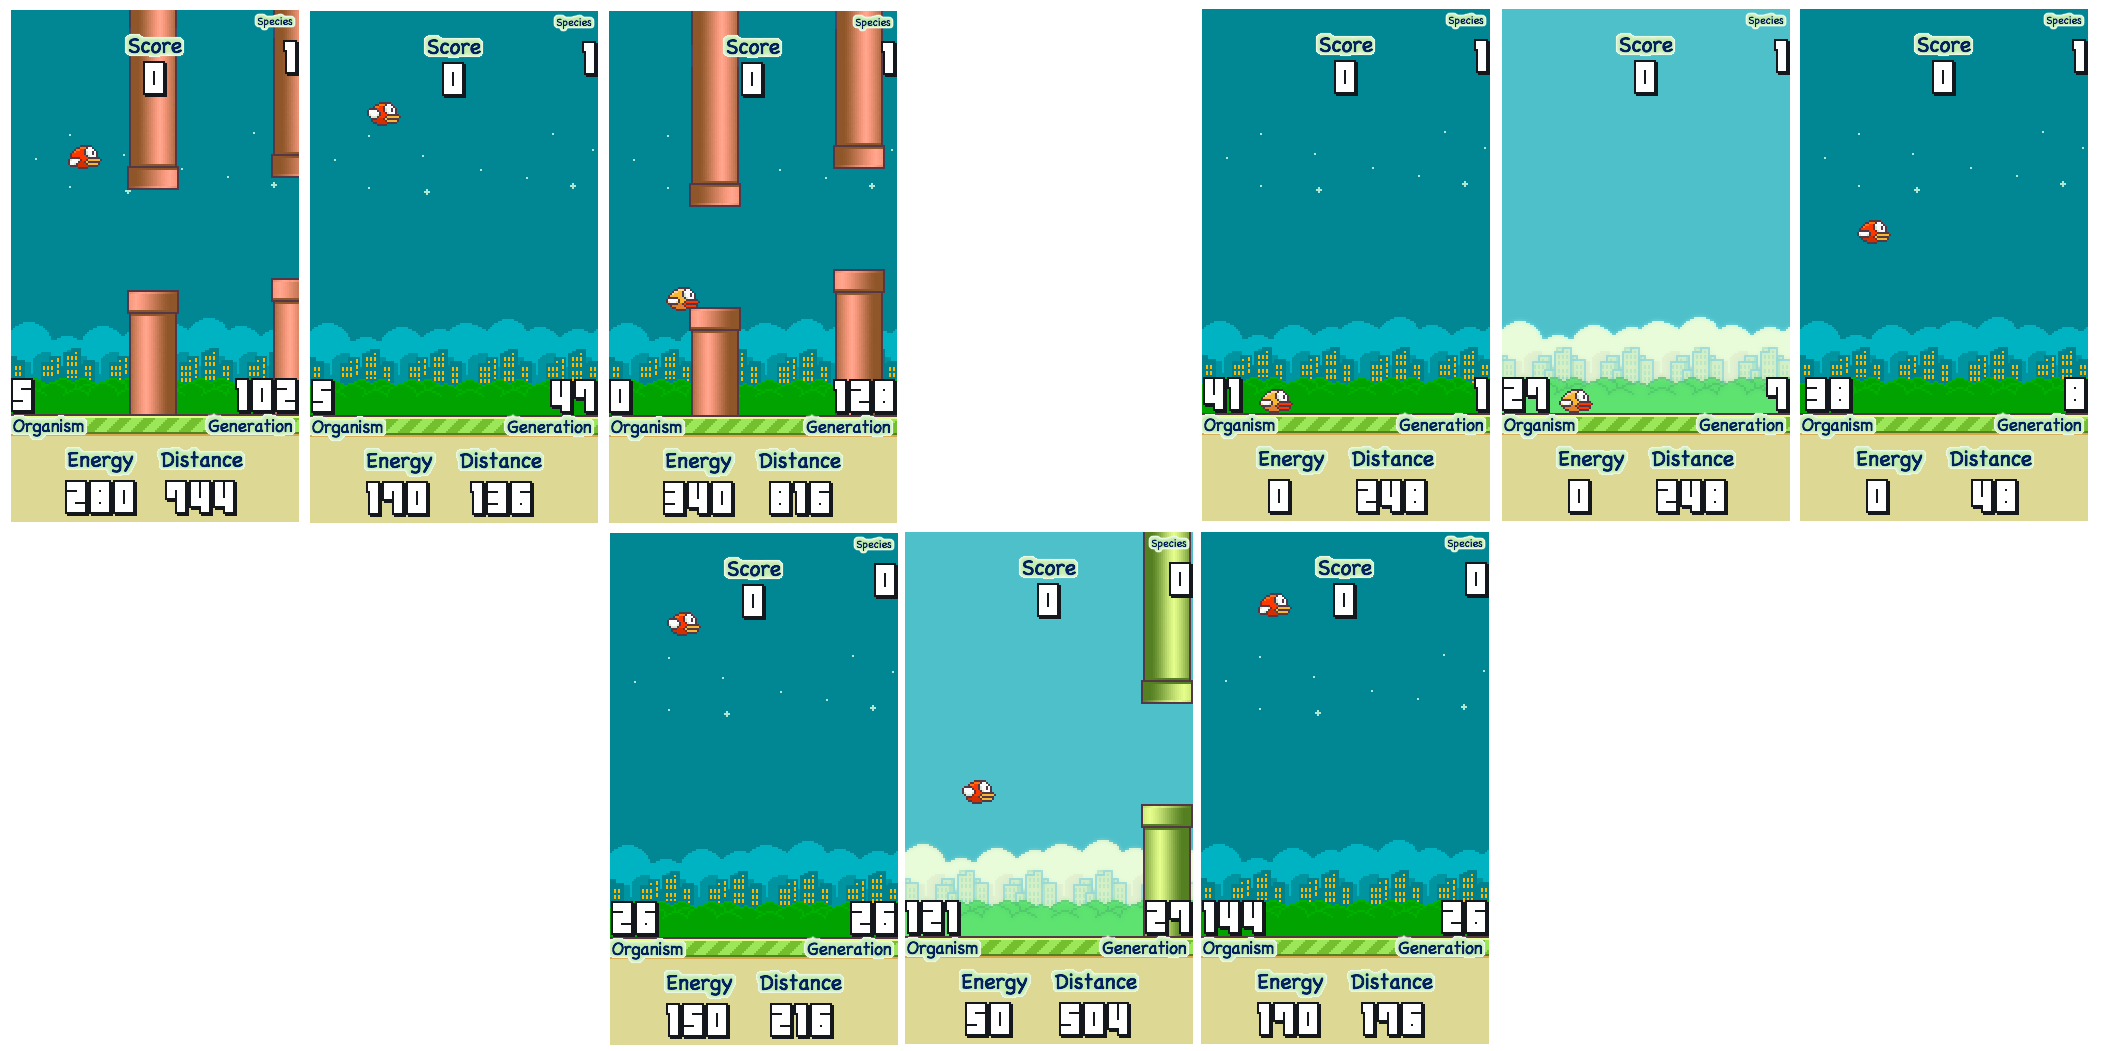
\includegraphics[width=1\textwidth]{graphics/flappy/flappy_sim_s1}
			\caption{Flappy Birds simulation}
		\end{figure}
		
		\begin{enumerate}
			\item explanation of environment and expectations
			\item fitnessfunction, formlar?
			\item explanation of graph of population (10, 50, 250) averaged on generations (30 generations evenly choosen [equal spaces between generation numbers])  (abstract explanation)
			\item check if expectations of marI/O can confirm
			\item huge difference between best runs and majority of runs (extreme luck), => double graph
			\item Differences between runs 
			\item unexpectedly bad results
			\item => Neat vs other machine learning
			\begin{enumerate}
				\item Differences between runs (lucky runs with 4th champion generation)
			\end{enumerate}
		\end{enumerate}
		
		\paragraph{Population 10 / Generation 500}
			asdf
%			\begin{figure}[h!]
%				\centering
%				\begin{minipage}{0.33\textwidth}
%					\centering
%					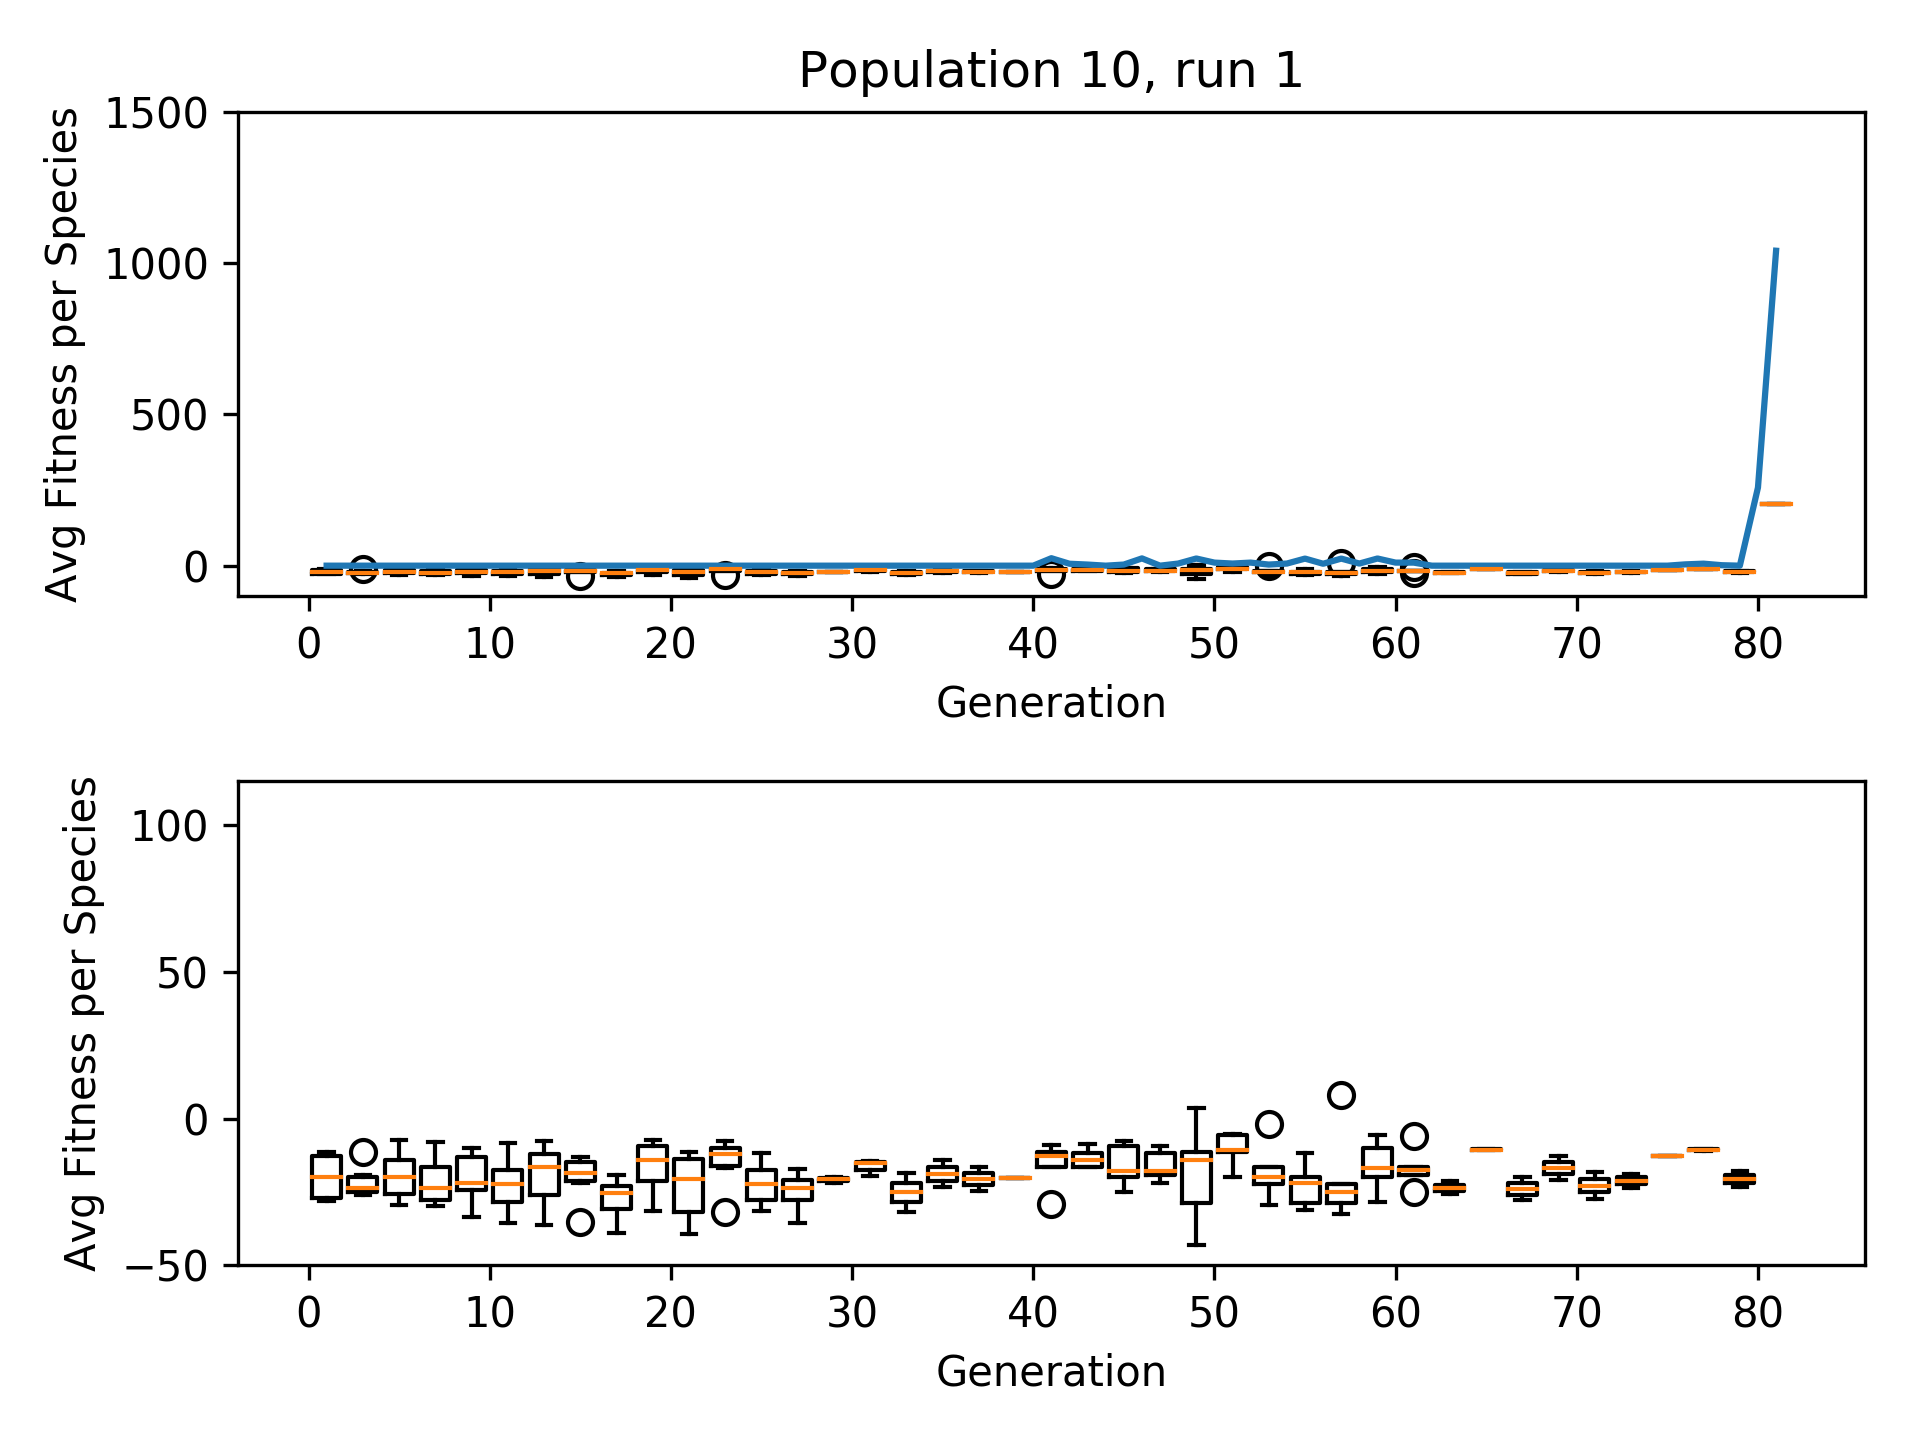
\includegraphics[width=1\textwidth]{graphics/flappy/pop10_run1} % first figure itself
%				\end{minipage}\hfill
%				\begin{minipage}{0.33\textwidth}
%					\centering
%					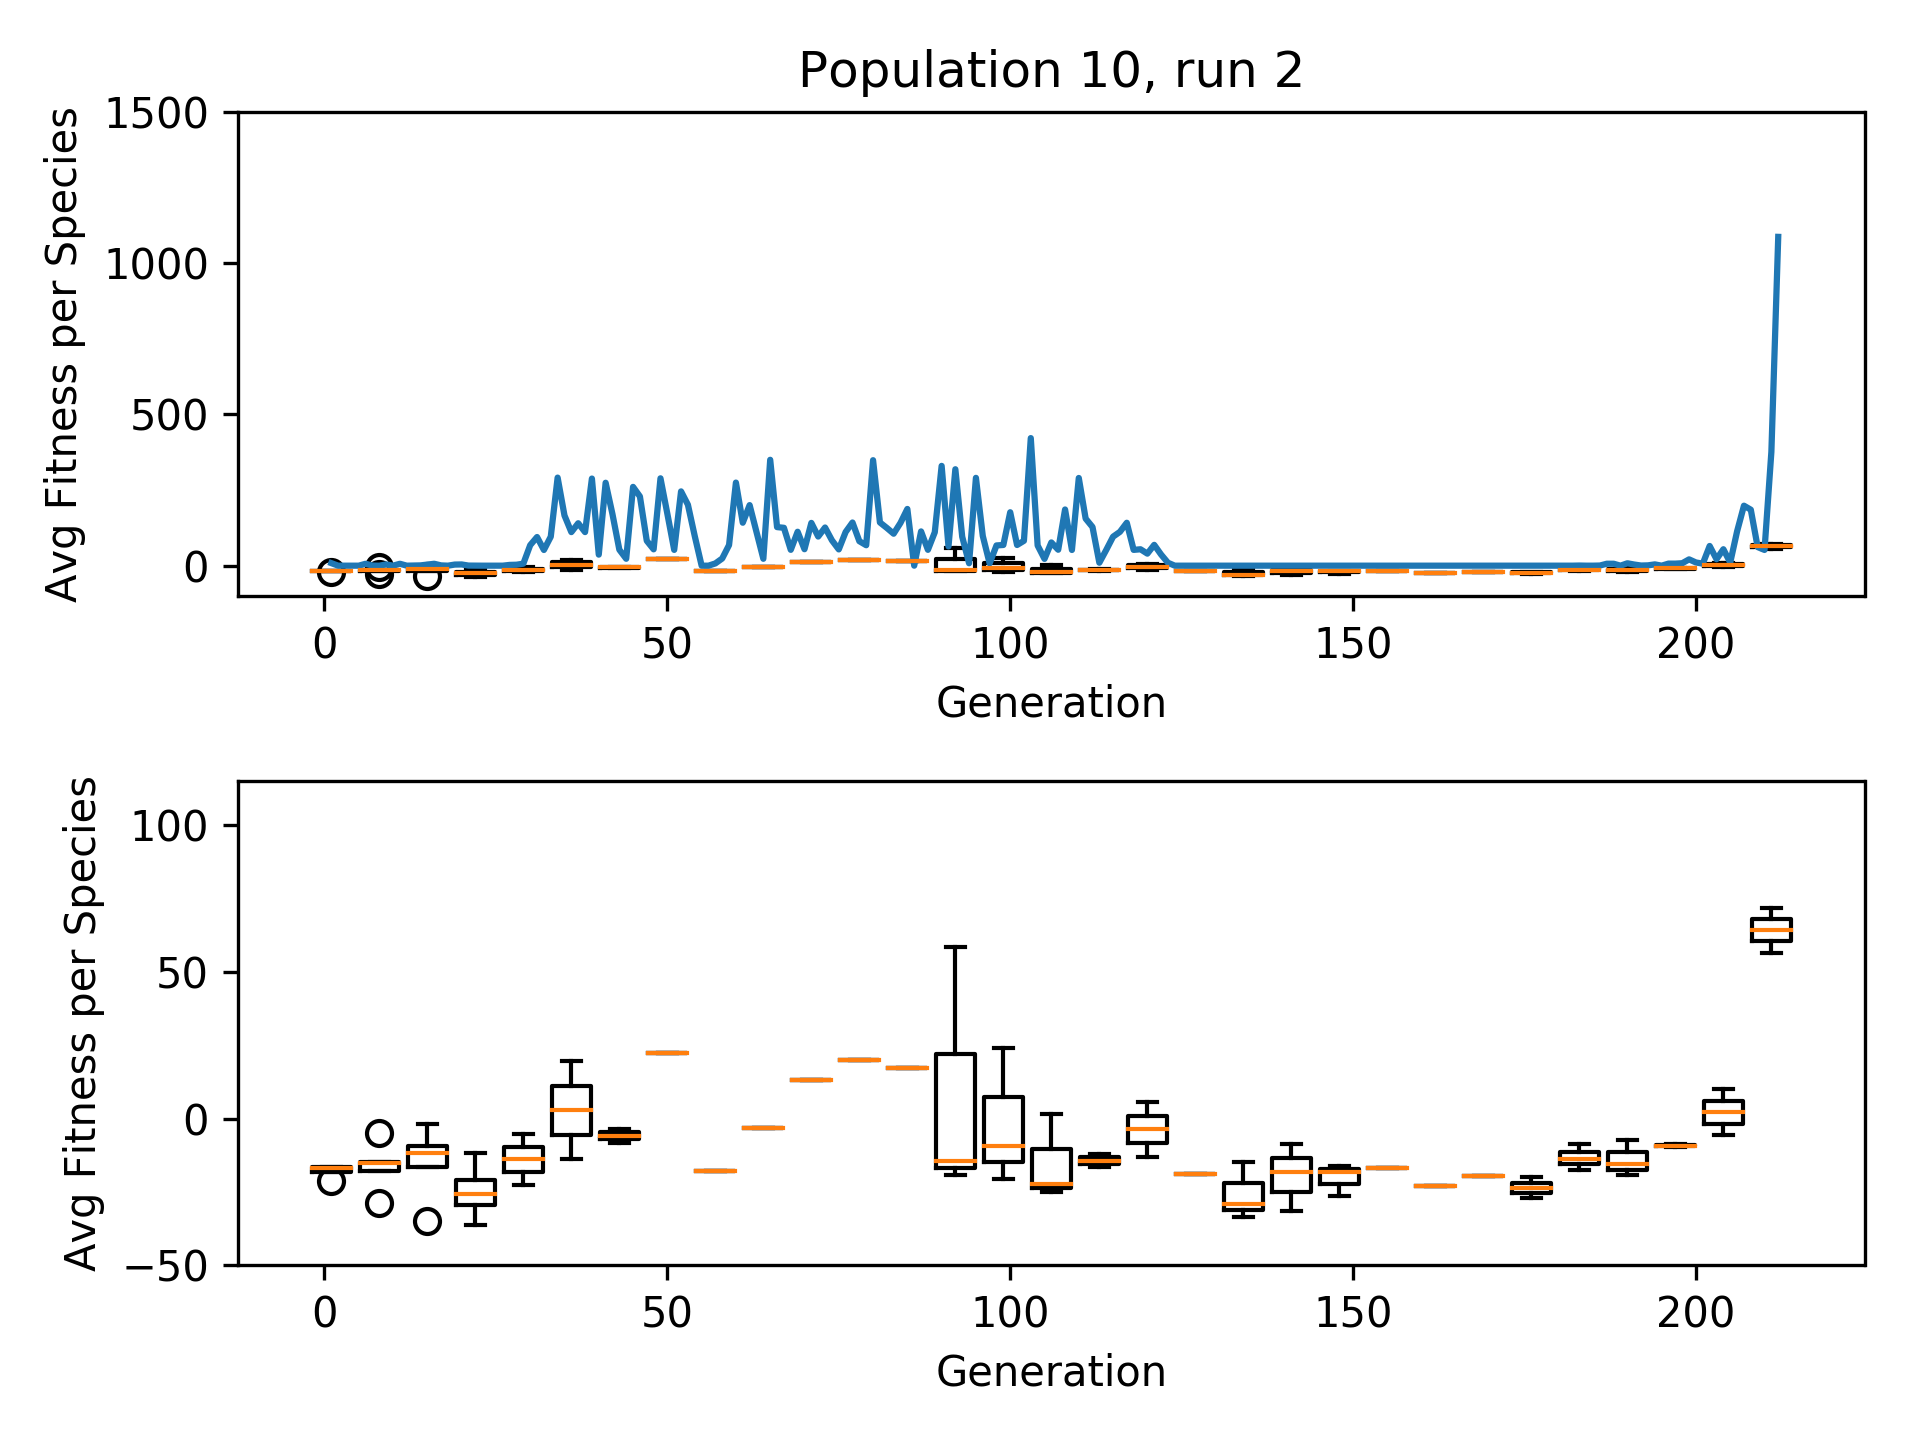
\includegraphics[width=1\textwidth]{graphics/flappy/pop10_run2} % second figure itself
%				\end{minipage}
%				\begin{minipage}{0.33\textwidth}
%					\centering
%					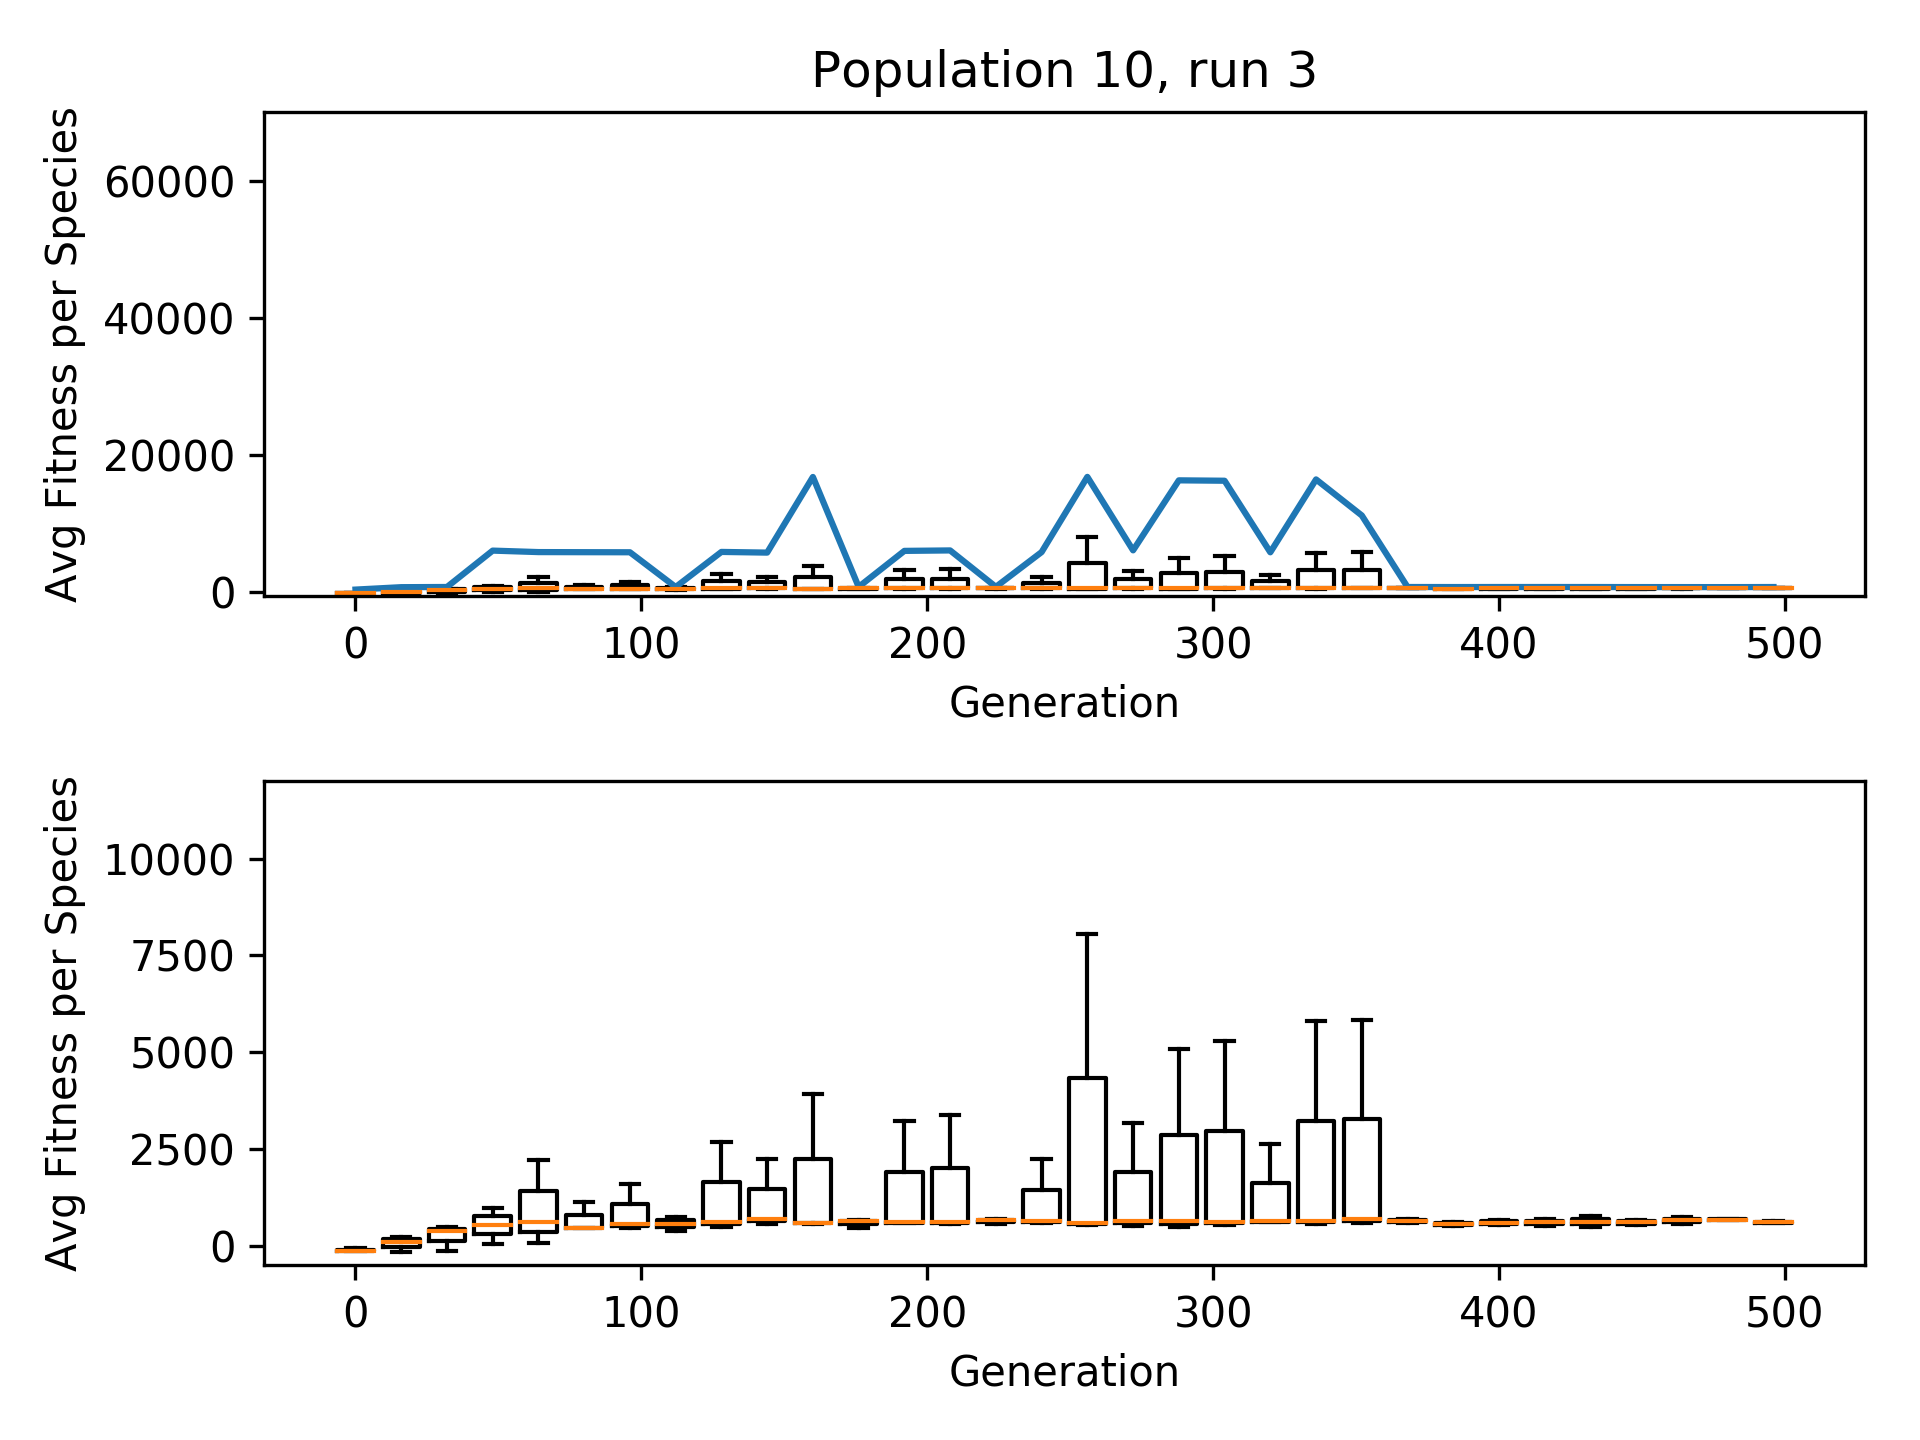
\includegraphics[width=1\textwidth]{graphics/flappy/pop10_run3} % second figure itself
%				\end{minipage}
%				\caption{Flappy Bird Population 10}
%			\end{figure}
		
		\paragraph{Population 50 / Generation 100}
			a
%			\begin{figure}[h]
%				\centering
%				\begin{minipage}{0.33\textwidth}
%					\centering
%					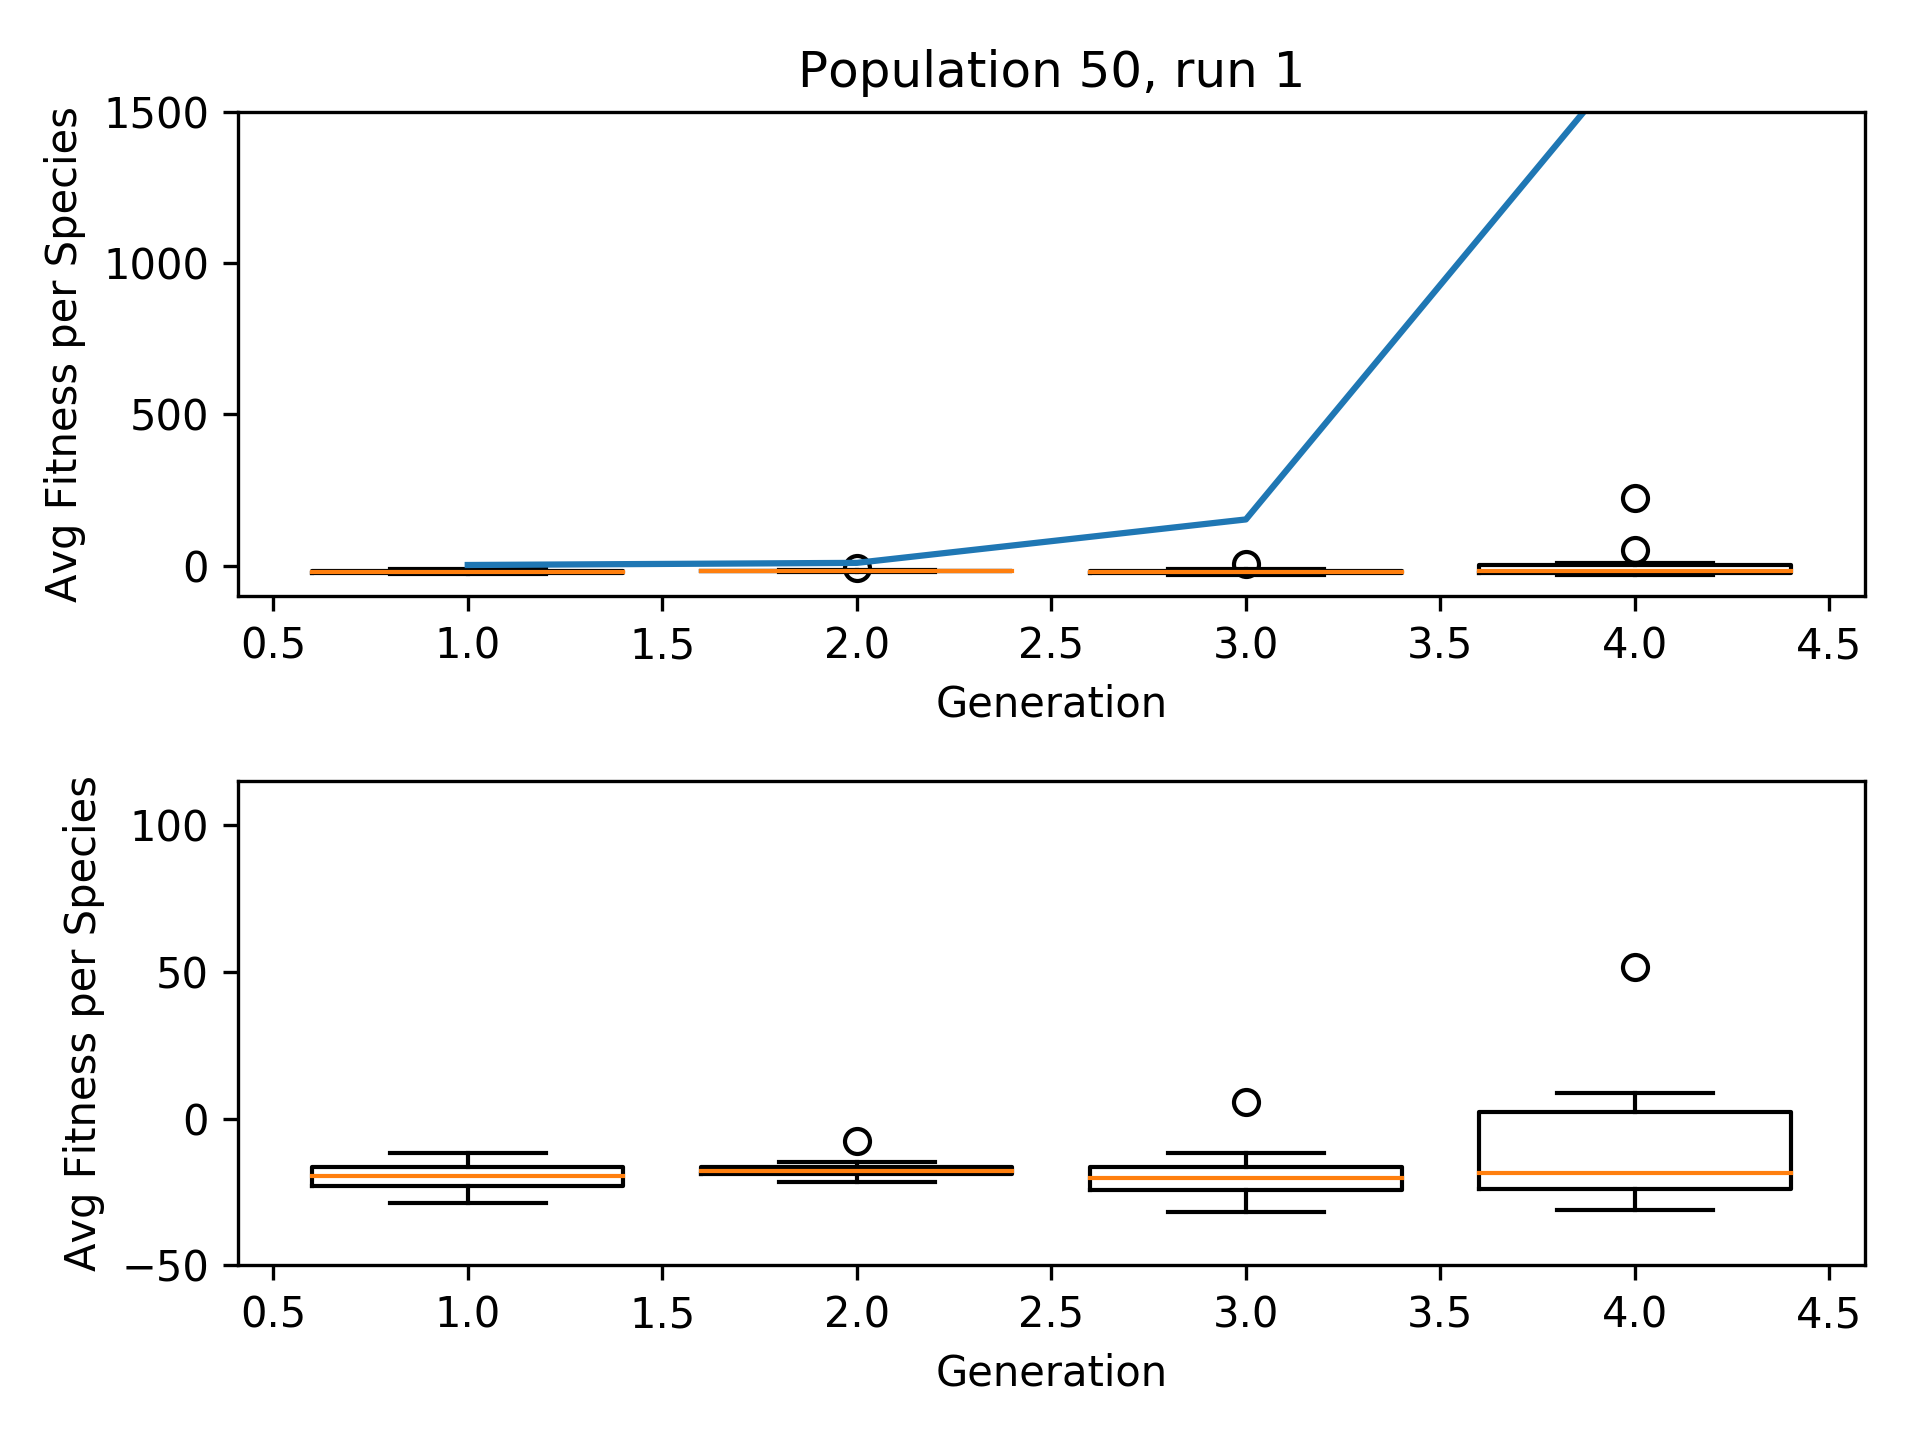
\includegraphics[width=1\textwidth]{graphics/flappy/pop50_run1} % first figure itself
%				\end{minipage}\hfill
%				\begin{minipage}{0.33\textwidth}
%					\centering
%					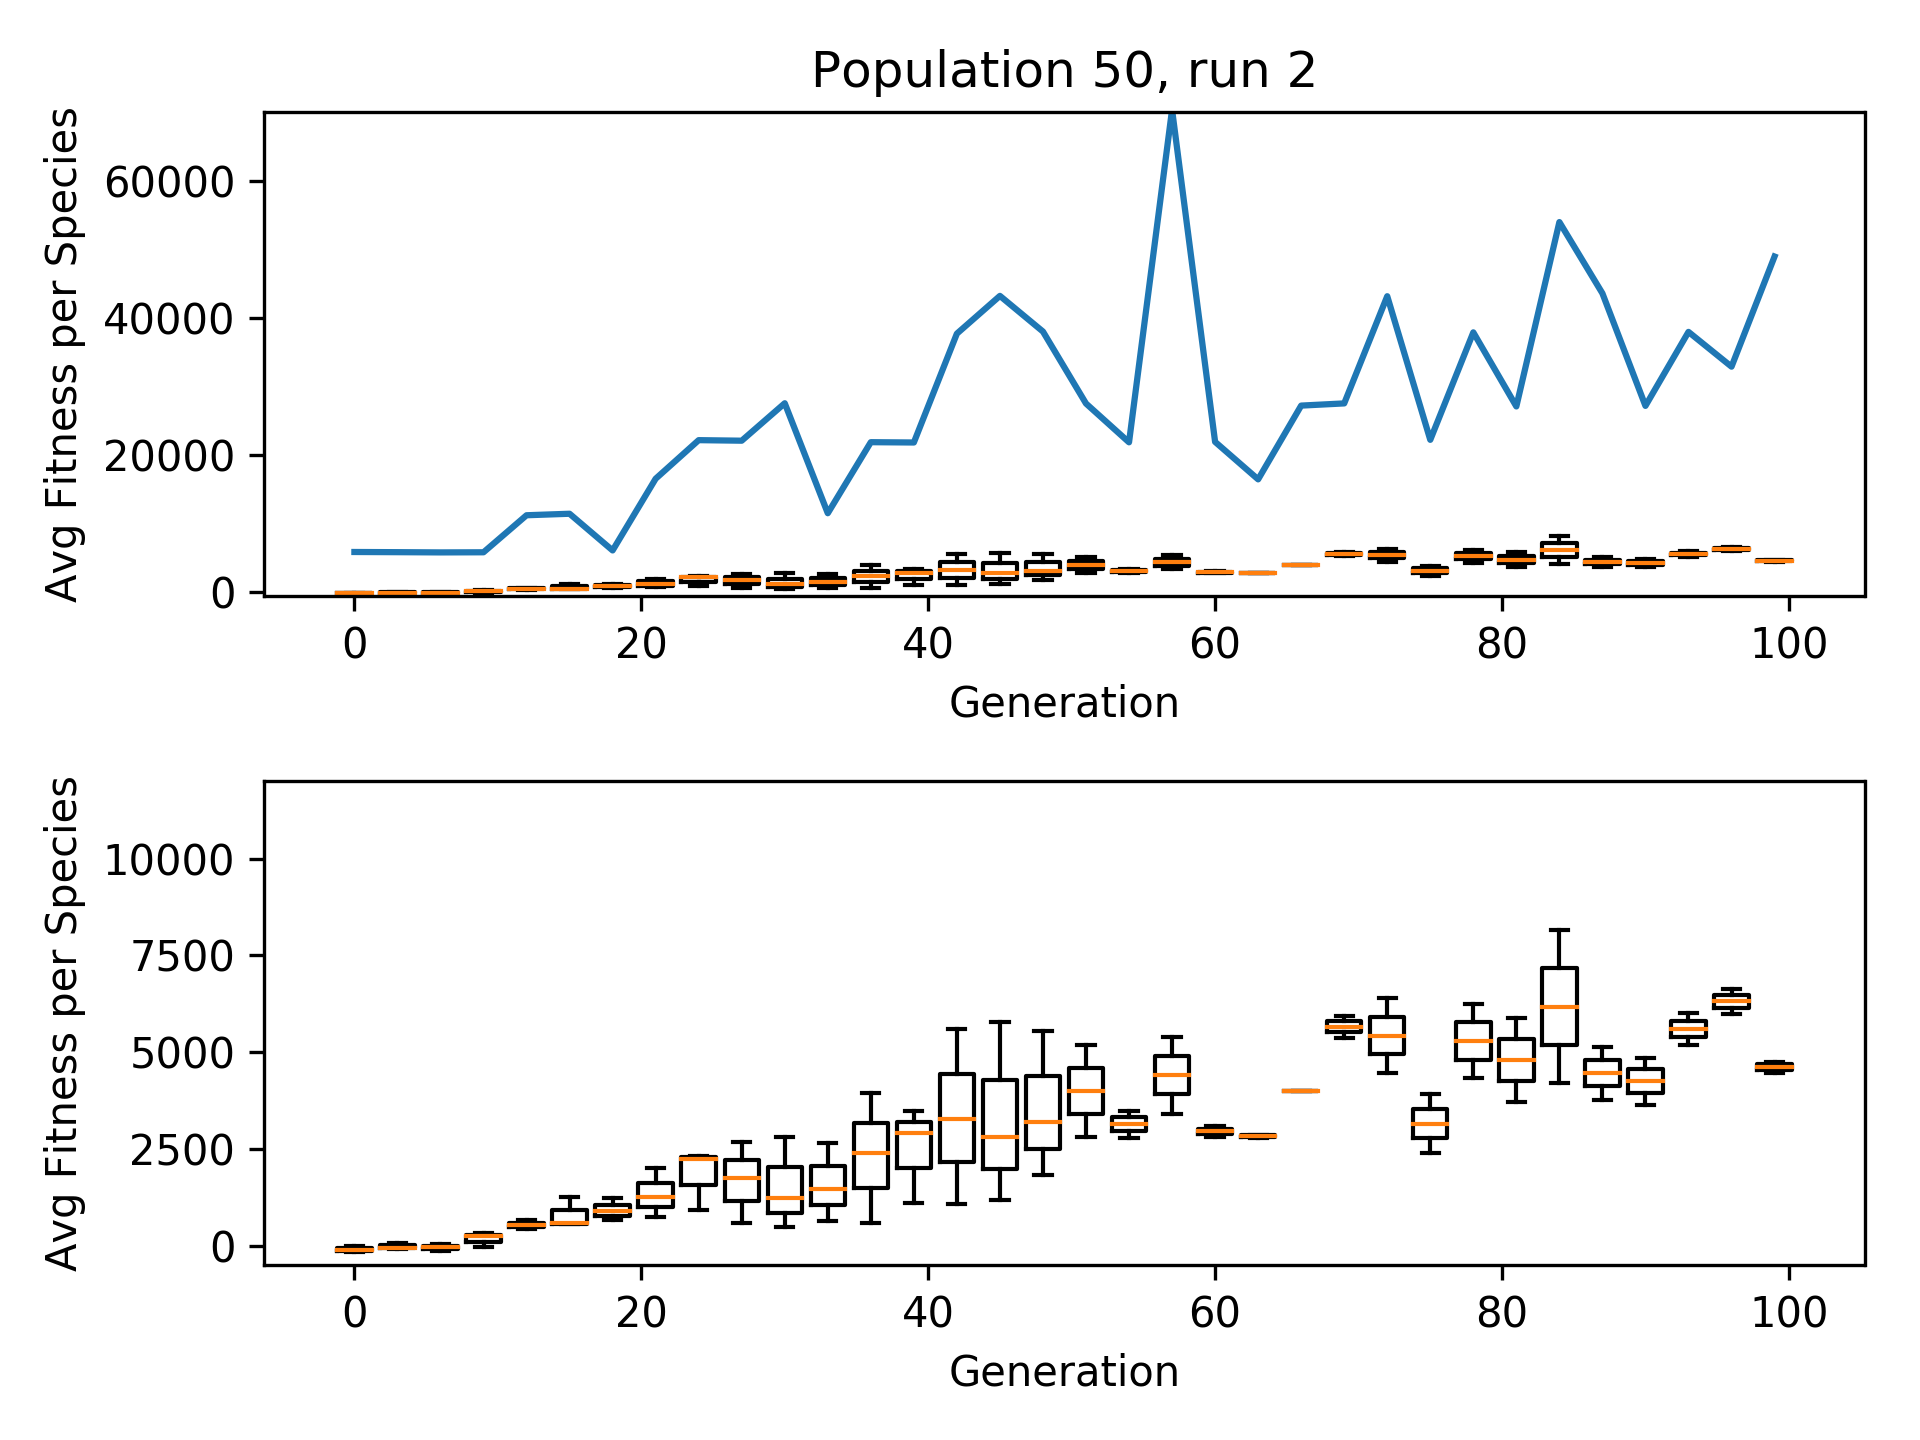
\includegraphics[width=1\textwidth]{graphics/flappy/pop50_run2} % second figure itself
%				\end{minipage}
%				\begin{minipage}{0.33\textwidth}
%					\centering
%					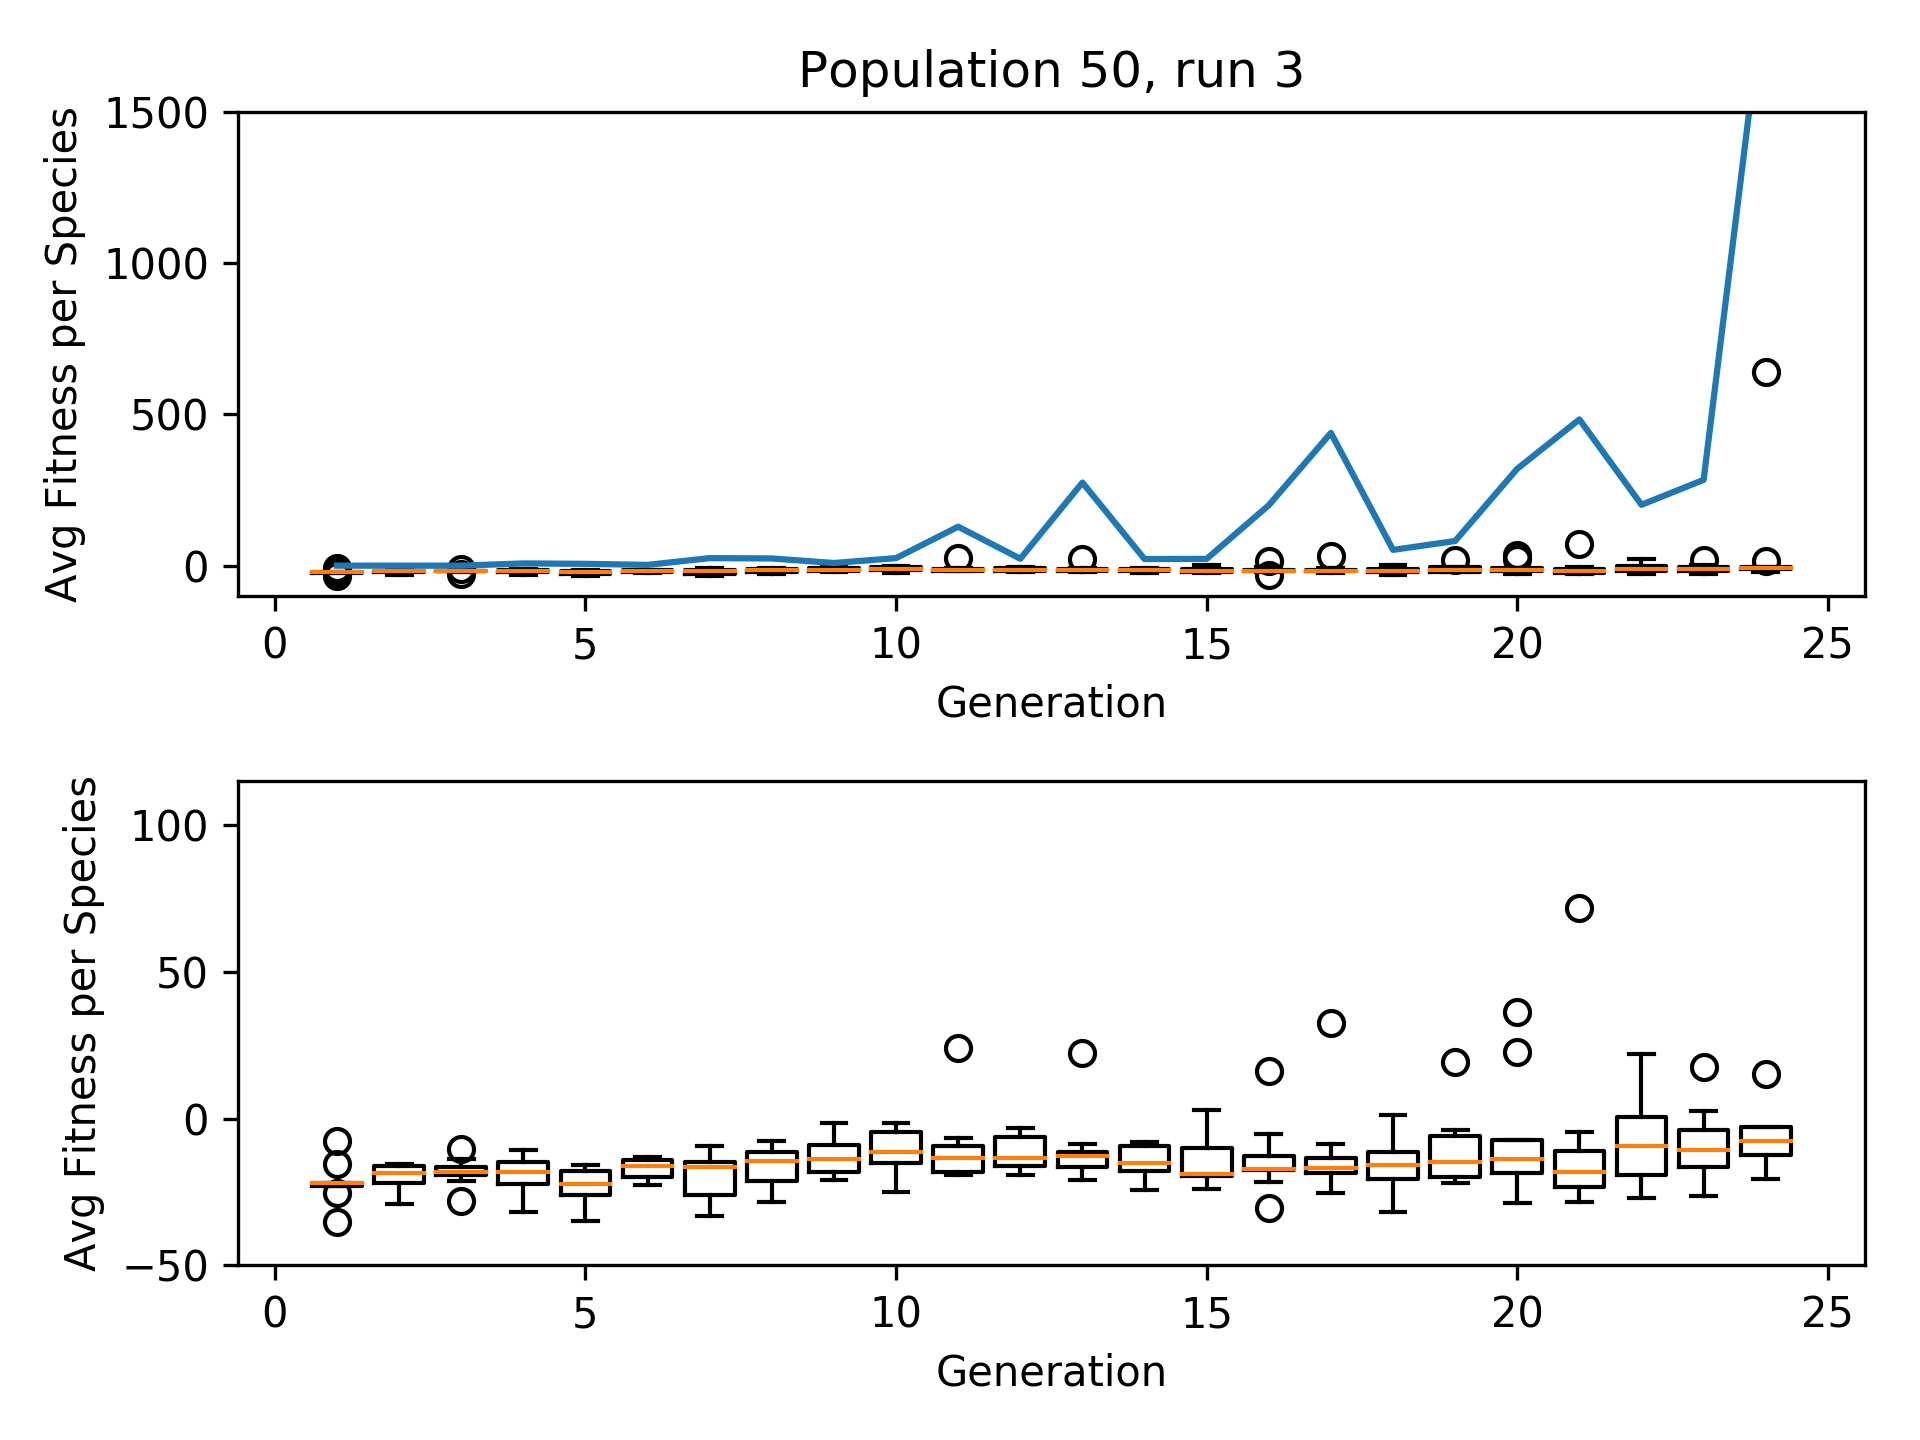
\includegraphics[width=1\textwidth]{graphics/flappy/pop50_run3} % second figure itself
%				\end{minipage}
%				\caption{Flappy Bird Population 50}
%			\end{figure}
		
		\paragraph{Population 250 / Generation 30}
		
			\begin{enumerate}
				\item best runs are exceptions (outside of whiskers)
			\end{enumerate}
			
%			\begin{figure}[h]
%				\centering
%				\begin{minipage}{0.33\textwidth}
%					\centering
%					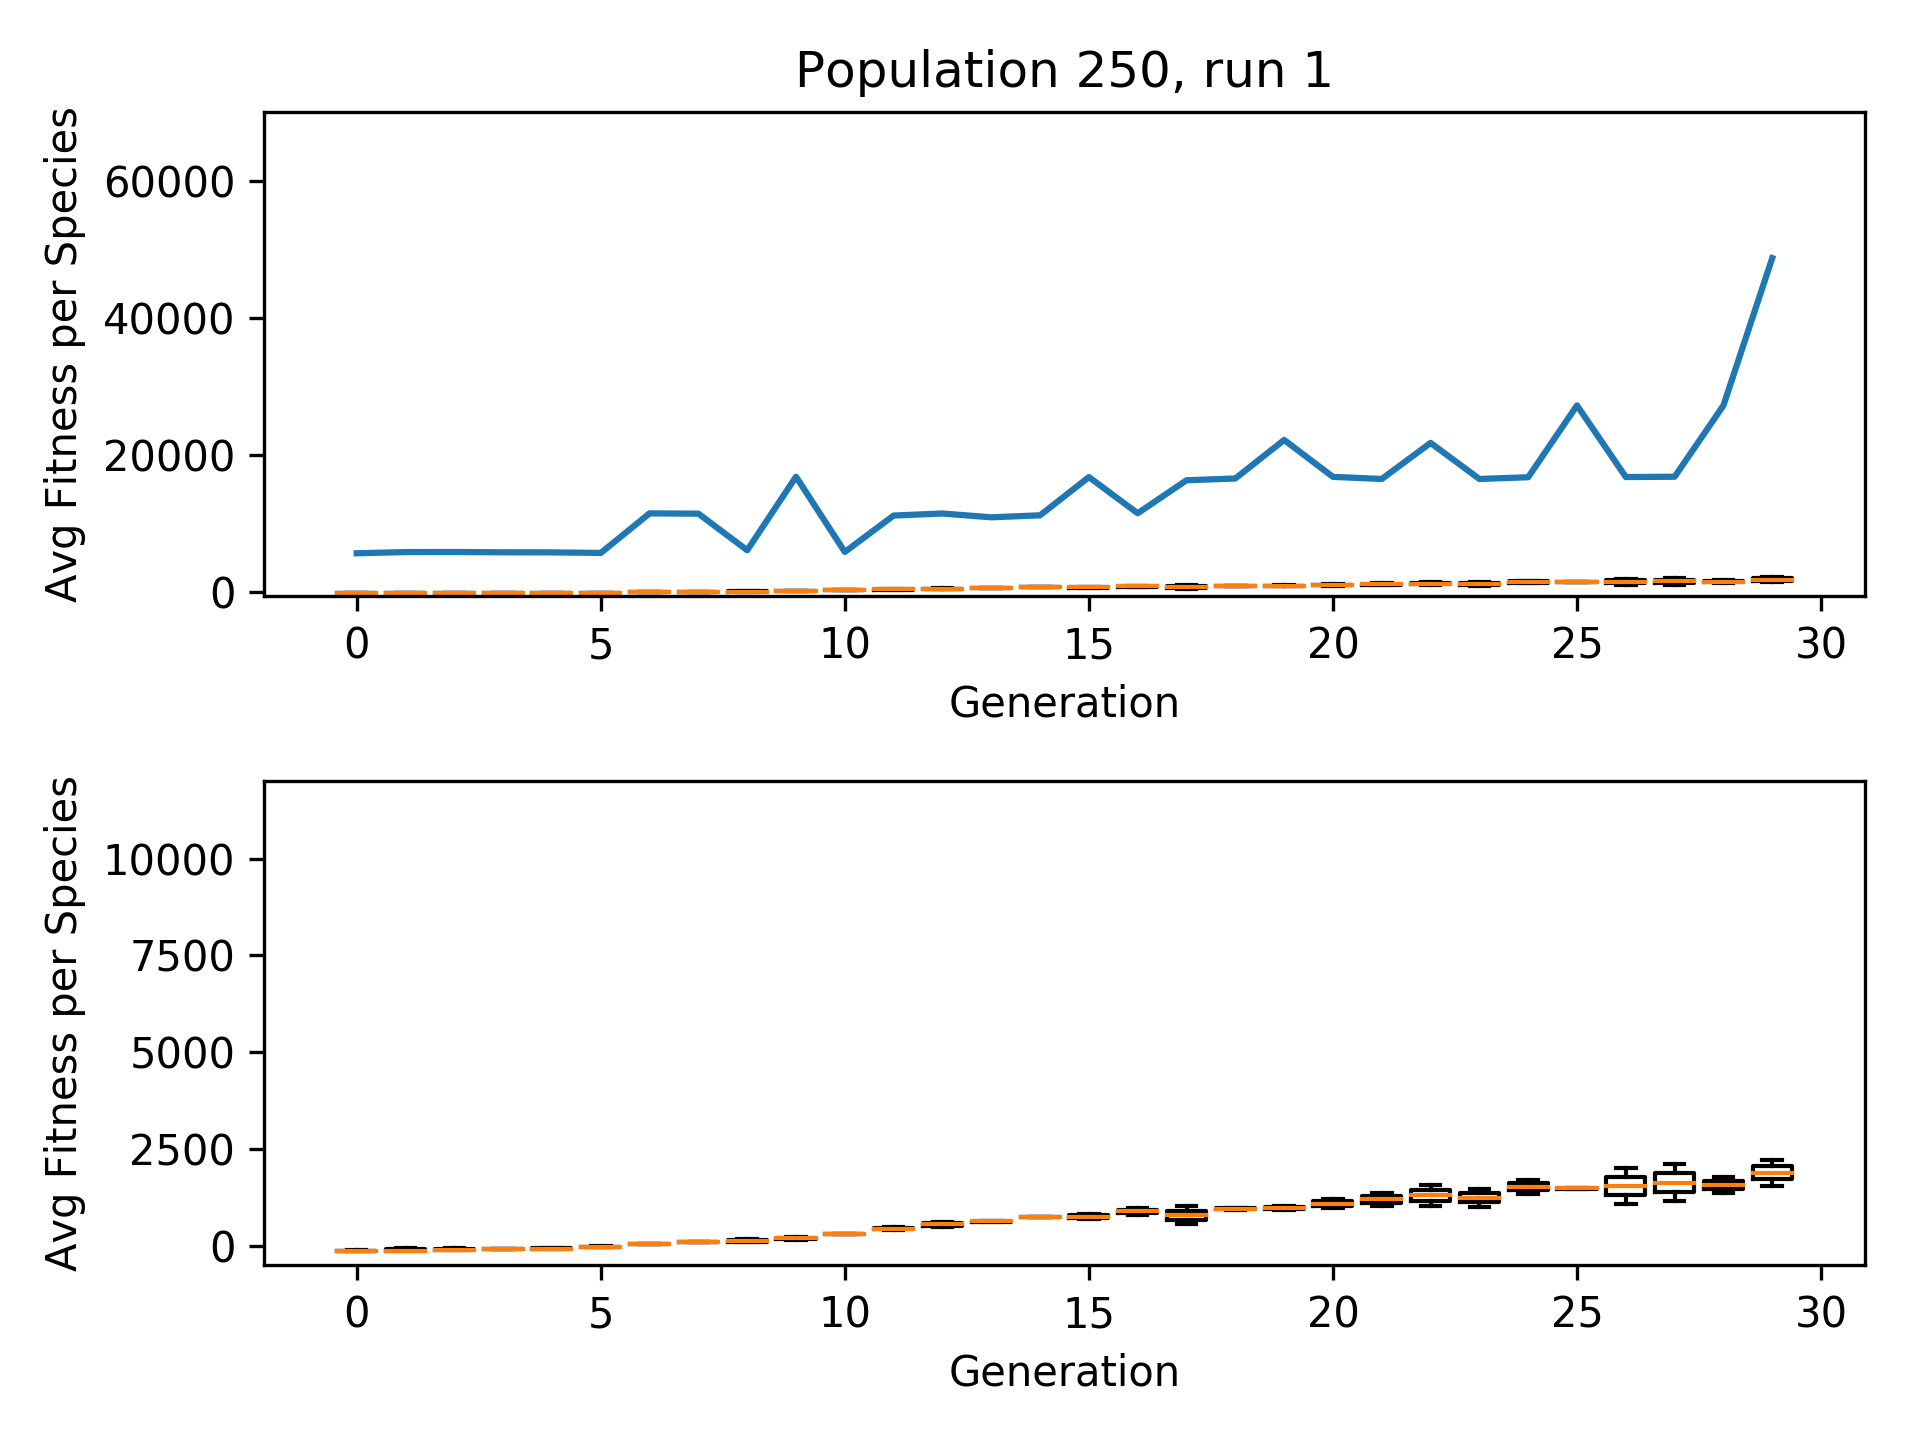
\includegraphics[width=1\textwidth]{graphics/flappy/pop250_run1} % first figure itself
%				\end{minipage}\hfill
%				\begin{minipage}{0.33\textwidth}
%					\centering
%					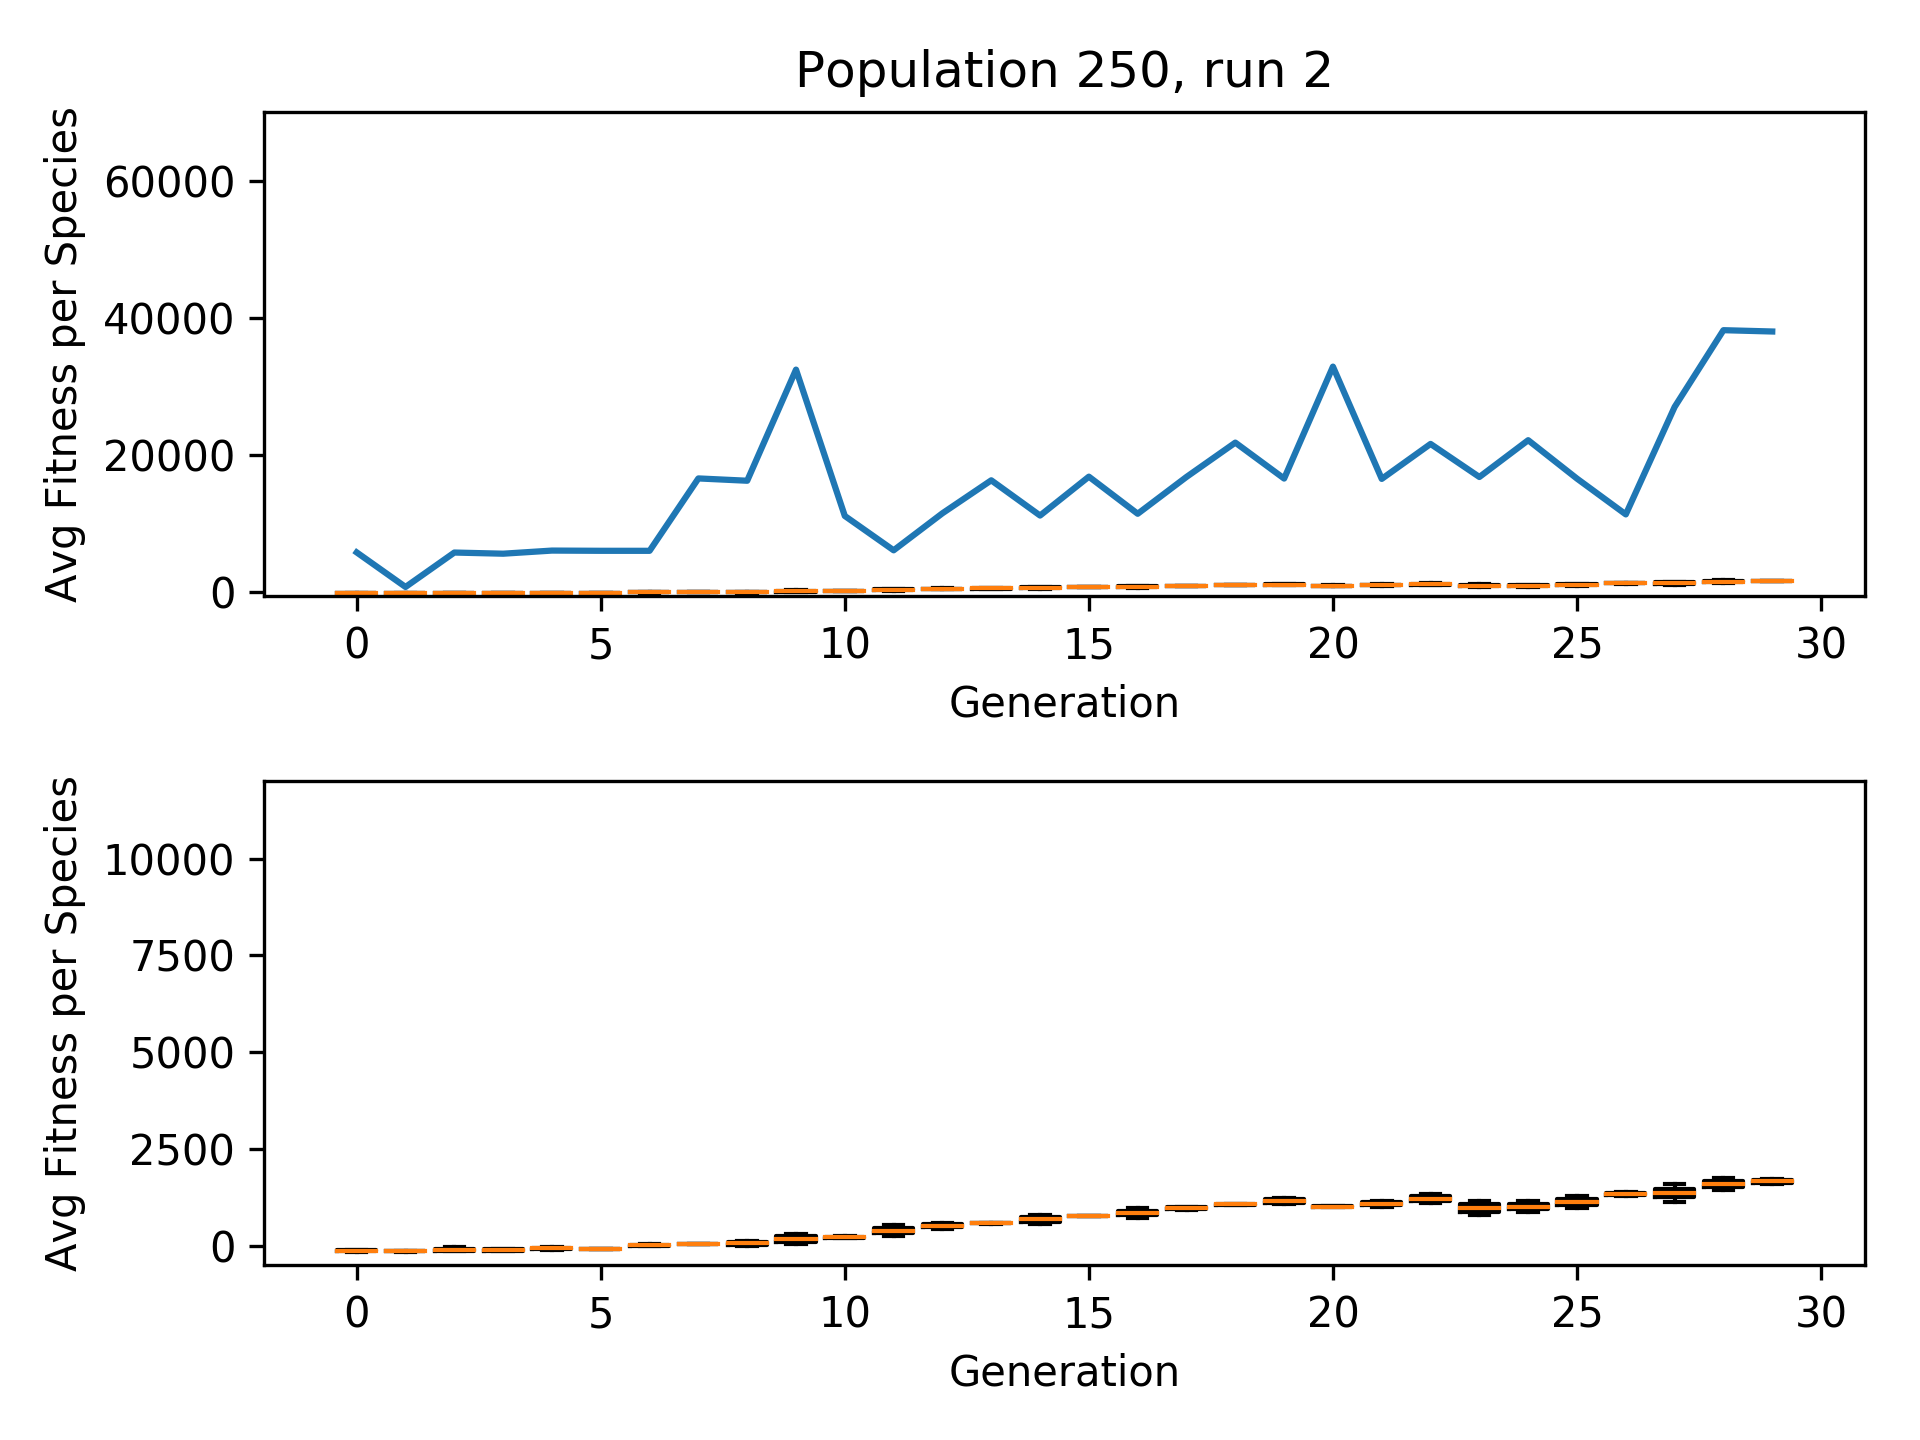
\includegraphics[width=1\textwidth]{graphics/flappy/pop250_run2} % second figure itself
%				\end{minipage}
%				\begin{minipage}{0.33\textwidth}
%					\centering
%					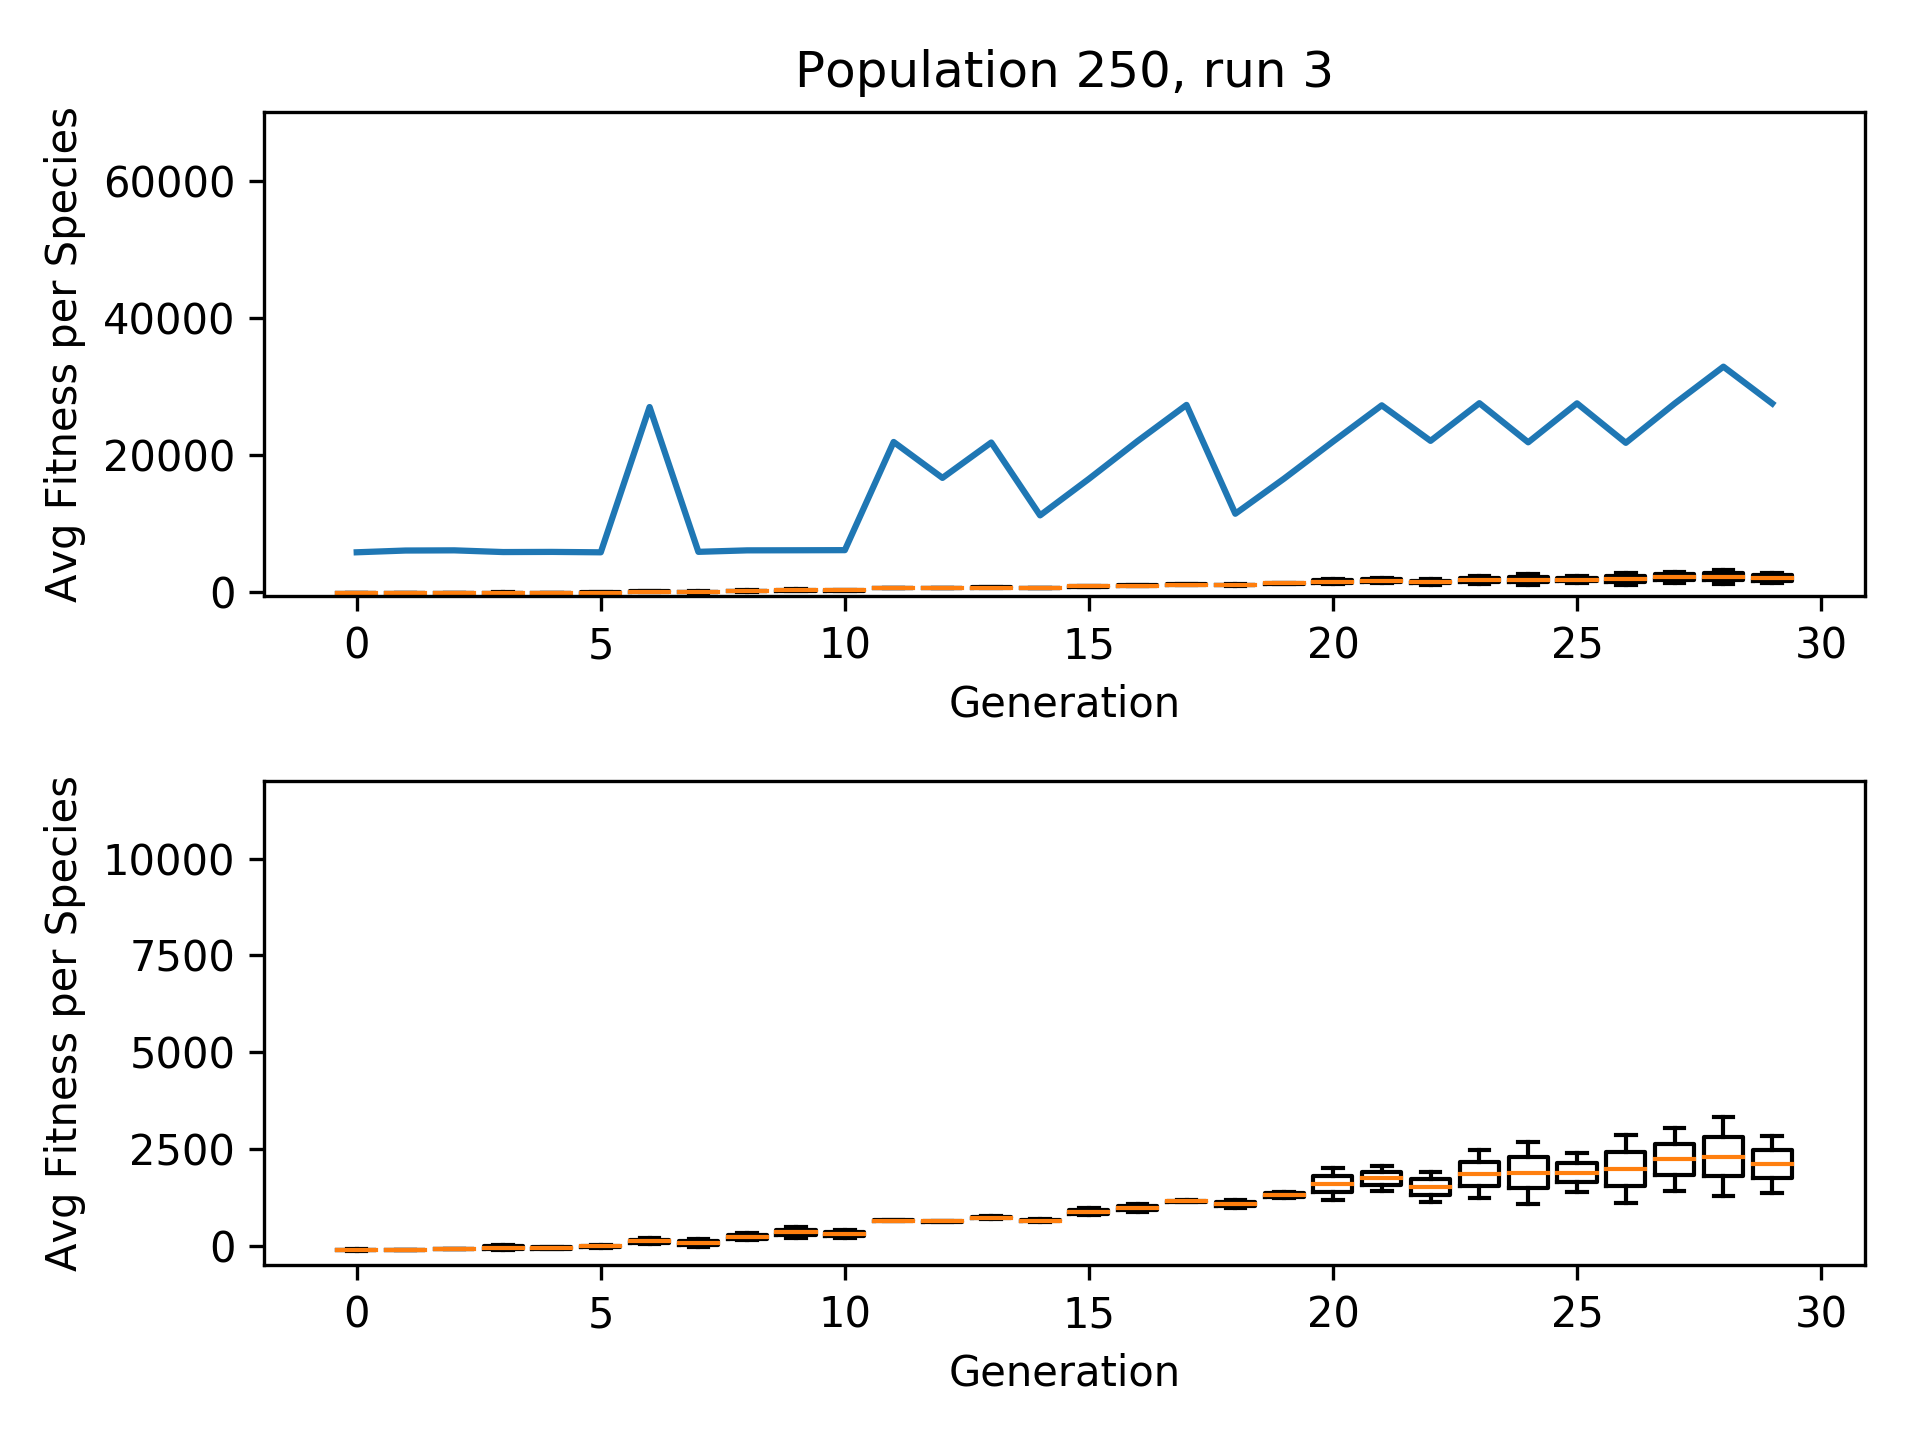
\includegraphics[width=1\textwidth]{graphics/flappy/pop250_run3} % second figure itself
%				\end{minipage}
%				\caption{Flappy Bird Population 250}
%			\end{figure}
		
		
		\subsection{Plain Machine learning flappy bird}
			\begin{enumerate}
				\item better results
				\item multi simulation made it easier
				\item easy algorithm for easy environment might be explanation for better results
			\end{enumerate}
	
	
	\section{Conclusion}
		\label{sec:system:conclusion}
		\begin{enumerate}
			\item differences / similarities in implementation (fixed size in machine learning flappy bird whereas dynamic species with marI/O)
			\item differences / similarities in outcome
			\item future studies
				\begin{itemize}
					\item genome/generation plot \& differences to other plot
					\item check in text for (future or further)
				\end{itemize}
		\end{enumerate}

         % INCLUDE: analysis
% !TEX root = ../thesis.tex


\chapter{Comparison and Meta-Analysis}
\label{sec:compare}

Much data was gathered and now we want to find out what this data indicates and how it can be used for future projects, maybe even real-world applications. 

\paragraph{Ignored Parameters}
\label{sec:compare:params}	
	In order to find a straight line for analyzing the data, many parameters were set by their default value. Other parameters have abstract meanings or simply define boundaries that didn't have to be considered. For example, in the configuration file of the \gls{neat} framework used in NEAT\_FlappyBird there are 63 lines of configuration.\\
	This complex set-up of the games leaves many wheels to turn and also give space to study their effect on the results systematically in future works. One starting-point can be the \gls{nn} parameters that were pre-specified for this simulations.\\
	Furthermore, the \gls{neat} implementations were not equal. First of all, they were written in two different programming/scripting languages. Furthermore, MarI/O was written from scratch and NEAT\_FlappyBird used a \gls{neat}-framework that allowed a high level of set-up-configurations and even self-implementations for various aspects of the algorithm. In this application only the default implementations were used as indicated by the following config initialization:
	\lstset{style=myPythonstyle} 
	\begin{lstlisting}[basicstyle=\small]
	config = neat.Config(neat.DefaultGenome, neat.DefaultReproduction, 
	neat.DefaultSpeciesSet, neat.DefaultStagnation, "config") 
	\end{lstlisting}
	However, despite the different set-up and configuration some similar results could be achieved using the \gls{neat} algorithm:

\section{Comparison of the different game environment}
\label{sec:compare:compare}	
	However, one parameter that was manipulated for this analyses is the initial population size. In MarI/O the initial population size spawned the defined amount of species with one genome each. In flappy bird, however, there were as many genomes launched as defined by the population size and after the run, they got assigned to their species.\\
	In order to display the differences in an overview, a table is presented containing the data trends. Despite their similarity, different fitness-functions have been taken to evaluate the success of a genome. This results in different scales in their values. That's why a more abstract indicator of the trend was chosen instead of the numbers. An arrow up ($\Big\uparrow$) indicates that the value was rising with a bigger initial population size and an arrow down ($\Big\downarrow$) indicates the opposite. When there is an $\bigtimes$ shown, it means that no trend could be found within the three population classes.
	\begin{table}[h]
		\centering
		\resizebox{\textwidth}{!}{
			\begin{tabular}[width=0.5\textwidth]{@{}ll|l|l|l|l@{}}
				\toprule
				Data Trend Comparison		& avg. runs /$\sigma$ 			& avg. fitness score /$\sigma$ 		& avg distance /$\sigma$ 		& avg. regress /$\sigma$ 			& avg. fitness increase /$\sigma$ 	\\ \midrule
				{\Large MarI/O} 			& $\Big\uparrow$ /$\times$      & $\Big\downarrow$ /$\downarrow$ 	& $\Big\uparrow$ /$\times$  	& $\Big\downarrow$ /$\downarrow$    & $\Big\uparrow$ /$\times$          \\
				{\Large NEAT\_FlappyBird}	& $\bigtimes$ /$\downarrow$    	& $\bigtimes$ /$\downarrow$ 		& $\Big\uparrow$ /$\times$  	& $\bigtimes$ /$\times$    			& $\Big\uparrow$ /$\times$          \\ \bottomrule
			\end{tabular}
		}
		\caption{Date Trend Comparison of different games and their \gls{neat} implementation}
		\label{tab:comp}
	\end{table} 
	At first, the differences are pointed out which are the following: 
	In MarI/O the average fitness score dropped with a bigger initial population. In NEAT\_FlappyBird there couldn't be a correlation drawn between the population size and the average fitness score.\\
	However, the standard deviation of the average fitness score dropped in both environments. This outcome is reasonable since there are fewer generations when the initial population size is larger.\\
	Further, in MarI/O the average regress (if present) becomes lower with bigger population sizes, as well as it's deviation. Interestingly, in NEAT\_FlappyBird no trend could be found at all since the population class had a higher average regress than the population class 10 but population class 250 didn't have any regress at all.\\
	The standard deviation of the average fitness increase had no trend in the NEAT\_FlappyBird implementation, however, it was quite similar in MarI/O's simulations. Still, the trend of the average fitness increase is the same in both simulations.
	
	When looking at the similarities of the results of the two environments there are two trends visible:
	One not so obvious correlation is that the distance of the median of the species to the best run of each generation is becoming greater with a greater population count. However, the standard deviation of this data is quite high in some cases. Still, in population class 250, the standard deviation was low when compared to the average regress value in MarI/O as well as NEAT\_FlappyBird.\\
	A more reasonable trend is that the population class 250 has a bigger average fitness increase than the other two simulation classes since the number of generations are smaller, although the goal/threshold was reached as well.\\
	When comparing the average distance with the average fitness increase, it can be seen that there are only a few genomes in the runs of population class 250 that reached a higher score, however, the majority of runs remained low. This division becomes larger the bigger the initial population size is. In MarI/O the average regress became lower with a higher population count, which indicates a certain stability. However, this stability could not be found in Flappy Bird. A reason for this can be the known bad performance of neat in extreme situations, since Flappy Bird has a randomly generated and therefore unknown world, whereas Super Mario World is deterministic in its level behavior\cite{kohl_integrated_2011}.
       % INCLUDE: comparison
% !TEX root = ../thesis.tex
%
\chapter{Conclusion}
\label{sec:conclusion}

\chapterprecishere{"By far, the greatest danger of Artificial Intelligence is that people conclude too early that they understand it."\par\raggedleft--- \textup{Eliezer S. Yudkowsky}, (Artificial Intelligence Researcher)}

% \cleanchapterquote{By far, the greatest danger of Artificial Intelligence is that people conclude too early that they understand it.}{Eliezer S. Yudkowsky}{(Artificial Intelligence Researcher)}

https://sokogskriv.no/en/writing/structure/structuring-a-thesis/
http://www.charleslipson.com/How-to-write-a-thesis.htm

\begin{itemize}
	\item 
	\item test MarI/O previous evolutions on other levels (long: what would be expected, how long to adapt to differences, would be better than start from anew)
	\item compare MarI\O to other solutions (see paper unofficial paper https://www.cs.cmu.edu/~tom7/mario/mario.pdf)
\end{itemize}


\section{Stuff}
\label{sec:conclusion:sec1}


\section{Future Work}
\label{sec:conclusion:future}

     % INCLUDE: conclusion\\

% \chapter{Additional Chapter}
% \todo{Enter your text here.}

% Remove following line for the final thesis.
% %% intro.tex
%% Copyright (C) 2014-2017 by Thomas Auzinger <thomas@auzinger.name>
%
% This work may be distributed and/or modified under the
% conditions of the LaTeX Project Public License, either version 1.3
% of this license or (at your option) any later version.
% The latest version of this license is in
%   http://www.latex-project.org/lppl.txt
% and version 1.3 or later is part of all distributions of LaTeX
% version 2005/12/01 or later.
%
% This work has the LPPL maintenance status `maintained'.
%
% The Current Maintainer of this work is Thomas Auzinger.
%
% This work consists of the files vutinfth.dtx and vutinfth.ins
% and the derived file vutinfth.cls.
% This work also consists of the file intro.tex.


\newacronym{ctan}{CTAN}{Comprehensive TeX Archive Network}
\newacronym{faq}{FAQ}{Frequently Asked Questions}
\newacronym{pdf}{PDF}{Portable Document Format}
\newacronym{svn}{SVN}{Subversion}
\newacronym{wysiwyg}{WYSIWYG}{What You See Is What You Get}

\newglossaryentry{texteditor}
{
  name={editor},
  description={A text editor is a type of program used for editing plain text files.}
}

\chapter{Introduction to \LaTeX}

Since \LaTeX\ is widely used in academia and industry, there exists a plethora of freely accessible introductions to the language.
Reading through the guide at \url{https://en.wikibooks.org/wiki/LaTeX} serves as a comprehensive overview for most of the functionality and is highly recommended before starting with a thesis in \LaTeX.

\section{Installation}

A full \LaTeX\ distribution\index{distribution} consists of not only of the binaries that convert the source files to the typeset documents, but also of a wide range of packages and their documentation.
Depending on the operating system, different implementations are available as shown in Table~\ref{tab:distrib}.
\textbf{Due to the large amount of packages that are in everyday use and due to their high interdependence, it is paramount to keep the installed distribution\index{distribution} up to date.}
Otherwise, obscure errors and tedious debugging ensue.

\begin{table}
  \centering
  \begin{tabular}{cccc}
    \toprule
    Distribution & Unix         & Windows      & MacOS        \\
    \midrule
    TeX Live     & \textbf{yes} & yes          & (yes)        \\
    MacTeX       & no           & no           & \textbf{yes} \\
    MikTeX       & no           & \textbf{yes} & no           \\
    \bottomrule
  \end{tabular}
  \caption{\TeX/\LaTeX\ distributions for different operating systems. Recomended choice in \textbf{bold}.}
  \label{tab:distrib} % \label has to be placed AFTER \caption to produce correct cross-references.
\end{table}

\section{Editors}

A multitude of \TeX\ \glspl{texteditor} are available differing in their editing models, their supported operating systems and their feature sets.
A comprehensive overview of \glspl{texteditor} can be found at the Wikipedia page  \url{https://en.wikipedia.org/wiki/Comparison_of_TeX_editors}.
TeXstudio (\url{http://texstudio.sourceforge.net/}) is recommended.
Most editors support the scrolling the typeset preview document to a location in the source document by \verb|Ctrl| clicking the location in the source document.

\section{Compilation}

Modern editors usually provide the compilation programs to generate \gls{pdf} documents and for most \LaTeX\ source files, this is sufficient.
More advanced \LaTeX\ functionality, such as glossaries and bibliographies, needs additional compilation steps, however.
It is also possible that errors in the compilation process invalidate intermediate files and force subsequent compilation runs to fail.
It is advisable to delete intermediate files (\verb|.aux|, \verb|.bbl|, etc.), if errors occur and persist.
All files that are not generated by the user are automatically regenerated.
To compile the current document, the steps as shown in Table~\ref{tab:compile} have to be taken.


\begin{table}
  \centering
  \begin{tabular}{rl}
    \toprule
    & Description \\
    \midrule
    1 & Scan for refs, toc/lof/lot/loa items and cites \\
    2 & Build the bibliography     \\
    3 & Link refs and build the toc/lof/lot/loa \\
    4 & Link the bibliography \\
    5 & Build the glossary \\
    6 & Build the acronyms \\
    7 & Build the index \\
    8 & Link the glossary, acronyms, and the index \\
    9 & Link the bookmarks \\
    \midrule
    & Command \\
    \midrule
    1 & \verb|pdflatex.exe  example| \\
    2 & \verb|bibtex.exe    example| \\
    3 & \verb|pdflatex.exe  example| \\
    4 & \verb|pdflatex.exe  example| \\
    5 & \verb|makeindex.exe -t example.glg -s example.ist| \\
      & \verb|              -o example.gls example.glo| \\
    6 & \verb|makeindex.exe -t example.alg -s example.ist| \\
      & \verb|              -o example.acr example.acn| \\
    7 & \verb|makeindex.exe -t example.ilg -o example.ind example.idx| \\
    8 & \verb|pdflatex.exe  example| \\
    9 & \verb|pdflatex.exe  example| \\
    \bottomrule
  \end{tabular}
  \caption{Compilation steps for this document. The following abbreviations were used: table of contents (toc), list of figures (lof), list of tables (lot), list of algorithms (loa).}
  \label{tab:compile} % \label has to be placed AFTER \caption to produce correct cross-references.
\end{table}


\section{Basic Functionality}

In this section, various examples are given of the fundamental building blocks used in a thesis.
Many \LaTeX\ commands have a rich set of options that can be supplied as optional arguments.
The documentation of each command should be consulted to get an impression of the full spectrum of its functionality.

\subsection{Floats}

Two main categories of page elements can be differentiated in the usual \LaTeX\ workflow: \textit{(i)} the main stream of text and \textit{(ii)} floating containers that are positioned at convenient positions throughout the document.
In most cases, tables, plots, and images are put into such containers since they are usually positioned at the top or bottom of pages.
These are realized by the two environments \verb|figure| and \verb|table|, which also provide functionality for cross-referencing (see Table~\ref{tab:intro} and Figure~\ref{fig:intro}) and the generation of corresponding entries in the list of figures and the list of tables.
Note that these environments solely act as containers and can be assigned arbitrary content.

\subsection{Tables}

A table in \LaTeX\ is created by using a \verb|tabular| environment or any of its extensions, e.g., \verb|tabularx|.
The commands \verb|\multirow| and \verb|\multicolumn| allow table elements to span multiple rows and columns.

\begin{table}[h] % placement specifier
  \centering
  \begin{tabular}{lll}
    \toprule
    \multicolumn{2}{c}{Position} \\
    \cmidrule{1-2} % partial horizontal rule
    Group & Abbrev & Name \\
    \midrule
    Goalkeeper & GK & Paul Robinson \\
    \midrule
    \multirow{4}{*}{Defenders} & LB & Lucus Radebe \\
                               & DC & Michael Duburry \\
                               & DC & Dominic Matteo \\
                               & RB & Didier Domi \\
    \midrule
    \multirow{3}{*}{Midfielders} & MC & David Batty \\
                                 & MC & Eirik Bakke \\
                                 & MC & Jody Morris \\
    \midrule
    Forward & FW & Jamie McMaster \\
    \midrule
    \multirow{2}{*}{Strikers} & ST & Alan Smith \\
                              & ST & Mark Viduka \\
    \bottomrule
  \end{tabular}
  \caption{Adapted example from the \LaTeX guide at \url{https://en.wikibooks.org/wiki/LaTeX/Tables}. This example uses rules specific to the \texttt{booktabs} package and employs the multi-row functionality of the \texttt{multirow} package.}
  \label{tab:intro} % \label has to be placed AFTER \caption to produce correct cross-references.
\end{table}

\subsection{Images}

An image is added to a document via the \verb|\includegraphics| command as shown in Figure~\ref{fig:intro}.
The \verb|\subcaption| command can be used to reference subfigures, such as Figure~\ref{fig:intro:full width} and~\ref{fig:intro:half width}.

\begin{figure}[h]
  \centering
  \begin{subfigure}[b]{0.45\columnwidth}
    \centering
    
\includegraphics[width=\textwidth]{TU_INF_Logo_gray}
    \subcaption{The header logo at text width.}
    \label{fig:intro:full width}
  \end{subfigure}
  \begin{subfigure}[b]{0.45\columnwidth}
    \centering
    
\includegraphics[width=0.5\textwidth]{TU_INF_Logo_gray}
    \subcaption{The header logo at half the text width.}
    \label{fig:intro:half width}
  \end{subfigure}
  \caption{The header logo at different sizes.}
  \label{fig:intro} % \label has to be placed AFTER \caption (or \subcaption) to produce correct cross-references.
\end{figure}

\subsection{Mathematical Expressions}

One of the original motivation to create the \TeX\ system was the need for mathematical typesetting.
To this day, \LaTeX\ is the preferred system to write math-heavy documents and a wide variety of functions aids the author in this task.
A mathematical expression can be inserted inline as $\sum_{n=1}^{\infty} \frac{1}{n^2} = \frac{\pi^2}{6}$ outside of the text stream as \[ \sum_{n=1}^{\infty} \frac{1}{n^2} = \frac{\pi^2}{6} \] or as numbered equation with
\begin{equation}
\sum_{n=1}^{\infty} \frac{1}{n^2} = \frac{\pi^2}{6}.
\end{equation}

\subsection{Pseudo Code}

The presentation of algorithms can be achieved with various packages; the most popular are \verb|algorithmic|, \verb|algorithm2e|, \verb|algorithmicx|, or \verb|algpseudocode|.
An overview is given at \url{https://tex.stackexchange.com/questions/229355}.
An example of the use of the \verb|alogrithm2e| package is given with Algorithm~\ref{alg:gauss-seidel}.

\begin{algorithm}
  \SetKw{BreakFor}{break for}
  \KwIn{A scalar~$\epsilon$, a matrix $\mathbf{A} = (a_{ij})$, a vector $\vec{b}$, and an initial vector $\vec{x}^{(0)}$}
  \KwOut{$\vec{x}^{(n)}$ with $\mathbf{A} \vec{x}^{(n)} \approx \vec{b}$}
  \For{$k\leftarrow 1$ \KwTo maximum iterations}
  {
     \For{$i\leftarrow 1$ \KwTo $n$}
     {
        $x_i^{(k)} = \frac{1}{a_{ii}} \left(b_i-\sum_{j<i} a_{ij} x_j^{(k)} - \sum_{j>i} a_{ij} x_j^{(k-1)} \right)$\;
     }
     \If{$\lvert\vec{x}^{(k)}-\vec{x}^{(k-1)}\rvert < \epsilon$}
     {\BreakFor\;}
  }
  \Return{$\vec{x}^{(k)}$\;}
  \caption{Gauss-Seidel}
  \label{alg:gauss-seidel} % \label has to be placed AFTER \caption to produce correct cross-references.
\end{algorithm}

\section{Bibliography}

The referencing of prior work is a fundamental requirement of academic writing and well supported by \LaTeX.
The \textsc{Bib}\TeX\ reference management software is the most commonly used system for this purpose.
Using the \verb|\cite| command, it is possible to reference entries in a \verb|.bib| file out of the text stream, e.g., as~\cite{Turing1936}.
The generation of the formatted bibliography needs a separate execution of \verb|bibtex.exe| (see Table~\ref{tab:compile}).

\section{Table of Contents}

The table of contents is automatically built by successive runs of the compilation, e.g., of \verb|pdflatex.exe|.
The command \verb|\setsecnumdepth| allows the specification of the depth of the table of contents and additional entries can be added to the table of contents using \verb|\addcontentsline|.
The starred versions of the sectioning commands, i.e., \verb|\chapter*|, \verb|\section*|, etc., remove the corresponding entry from the table of contents.

\section{Acronyms / Glossary / Index}

The list of acronyms, the glossary, and the index need to be built with a separate execution of \verb|makeindex| (see Table~\ref{tab:compile}).
Acronyms have to be specified with \verb|\newacronym| while glossary entries use \verb|\newglossaryentry|.
Both are then used in the document content with one of the variants of \verb|\gls|, such as \verb|\Gls|, \verb|\glspl|, or \verb|\Glspl|.
Index items are simply generated by placing \verb|\index|\marg{entry} next to all the words that correspond to the index entry \meta{entry}.
Note that many enhancements exist for these functionalities and the documentation of the \verb|makeindex| and the \verb|glossaries| packages should be consulted.

\section{Tips}

Since \TeX\ and its successors do not employ a \gls{wysiwyg} editing scheme, several guidelines improve the readability of the source content:
\begin{itemize}
\item Each sentence in the source text should start with a new line.
      This helps not only the user navigation through the text, but also enables revision control systems (e.g. \gls{svn}, Git) to show the exact changes authored by different users.
      Paragraphs are separated by one (or more) empty lines.
\item Environments, which are defined by a matching pair of \verb|\begin{name}| and \verb|\end{name}|, can be indented by whitespace to show their hierarchical structure.
\item In most cases, the explicit use of whitespace (e.g. by adding \verb|\hspace{4em}| or \verb|\vspace{1.5cm}|) violates typographic guidelines and rules.
      Explicit formatting should only be employed as a last resort and, most likely, better ways to achieve the desired layout can be found by a quick web search.
\item The use of bold or italic text is generally not supported by typographic considerations and the semantically meaningful \verb|\emph{|\texttt{$\dots$}\verb|}| should be used.
\end{itemize}

The predominant application of the \LaTeX\ system is the generation of \gls{pdf} files via the \textsc{Pdf}\LaTeX\ binaries.
In the current version of \textsc{Pdf}\LaTeX, it is possible that absolute file paths and user account names are embedded in the final \gls{pdf} document.
While this poses only a minor security issue for all documents, it is highly problematic for double blind reviews.
The process shown in Table~\ref{tab:ps2pdf} can be employed to strip all private information from the final \gls{pdf} document.

\begin{table}[h]
  \centering
  \begin{tabular}{rl}
  \toprule
  & Command \\
  \midrule
  1 & Rename the \gls{pdf} document \verb|final.pdf| to \verb|final.ps|. \\
  2 & Execute the following command: \\
    & \verb|ps2pdf -dPDFSETTINGS#/prepress ^| \\
    & \verb| -dCompatibilityLevel#1.4 ^| \\
    & \verb| -dAutoFilterColorImages#false ^| \\
    & \verb| -dAutoFilterGrayImages#false ^| \\
    & \verb| -dColorImageFilter#/FlateEncode ^| \\
    & \verb| -dGrayImageFilter#/FlateEncode ^| \\
    & \verb| -dMonoImageFilter#/FlateEncode ^| \\
    & \verb| -dDownsampleColorImages#false ^| \\
    & \verb| -dDownsampleGrayImages#false ^| \\
    & \verb| final.ps final.pdf| \\
  \bottomrule
  \end{tabular}

  On Unix-based systems, replace \verb|#| with \verb|=| and \verb|^| with \verb|\|.
  \caption{Anonymization of \gls{pdf} documents.}
  \label{tab:ps2pdf}
\end{table}

\section{Resources}

\subsection{Useful Links}

In the following, a listing of useful web resources is given.
\begin{description}
\item[\url{https://en.wikibooks.org/wiki/LaTeX}] An extensive wiki-based guide to \LaTeX.
\item[\url{http://www.tex.ac.uk/faq}] A (huge) set of \gls{faq} about \TeX\ and \LaTeX.
\item[\url{https://tex.stackexchange.com/}] The definitive user forum for non-trivial \LaTeX-related questions and answers.
\end{description}

\subsection[Comprehensive TeX Archive Network]{\gls{ctan}}

The \gls{ctan} is the official repository for all \TeX\ related material.
It can be accessed via \url{https://www.ctan.org/} and hosts (among other things) a huge variety of packages that provide extended functionality for \TeX\ and its successors.
Note that most packages contain \gls{pdf} documentation that can be directly accessed via \gls{ctan}.

In the following, a short, non-exhaustive list of relevant \gls{ctan}-hosted packages is given together with their relative path.
\begin{description}[itemsep=0ex]
\item[\href{https://www.ctan.org/pkg/algorithm2e}{algorithm2e}] Functionality for writing pseudo code.
\item[\href{https://www.ctan.org/pkg/amsmath}{amsmath}] Enhanced functionality for typesetting mathematical expressions.
\item[\href{https://www.ctan.org/pkg/amsfonts}{amssymb}] Provides a multitude of mathematical symbols.
\item[\href{https://www.ctan.org/pkg/booktabs}{booktabs}] Improved typesetting of tables.
\item[\href{https://www.ctan.org/pkg/enumitem}{enumitem}] Control over the layout of lists (\verb|itemize|, \verb|enumerate|, \verb|description|).
\item[\href{https://www.ctan.org/pkg/fontenc}{fontenc}] Determines font encoding of the output.
\item[\href{https://www.ctan.org/pkg/glossaries}{glossaries}] Create glossaries and list of acronyms.
\item[\href{https://www.ctan.org/pkg/graphicx}{graphicx}] Insert images into the document.
\item[\href{https://www.ctan.org/pkg/inputenc}{inputenc}] Determines encoding of the input.
\item[\href{https://www.ctan.org/pkg/l2tabu}{l2tabu}] A description of bad practices when using \LaTeX.
\item[\href{https://www.ctan.org/pkg/mathtools}{mathtools}] Further extension of mathematical typesetting.
\item[\href{https://www.ctan.org/pkg/memoir}{memoir}] The document class on upon which the \verb|vutinfth| document class is based.
\item[\href{https://www.ctan.org/pkg/multirow}{multirow}] Allows table elements to span several rows.
\item[\href{https://www.ctan.org/pkg/pgfplots}{pgfplots}] Function plot drawings.
\item[\href{https://www.ctan.org/pkg/pgf}{pgf/TikZ}] Creating graphics inside \LaTeX\ documents.
\item[\href{https://www.ctan.org/pkg/subcaption}{subcaption}] Allows the use of subfigures and enables their referencing.
\item[\href{https://www.ctan.org/tex-archive/info/symbols/comprehensive/}{symbols/comprehensive}] A listing of around 5000 symbols that can be used with \LaTeX.
\item[\href{https://www.ctan.org/pkg/voss-mathmode}{voss-mathmode}] A comprehensive overview of typesetting mathematics in \LaTeX.
\item[\href{https://www.ctan.org/pkg/xcolor}{xcolor}] Allows the definition and use of colors.
\end{description} % A short introduction to LaTeX.

\backmatter

% Use an optional list of figures.
\listoffigures % Starred version, i.e., \listoffigures*, removes the toc entry.

% Use an optional list of tables.
\cleardoublepage % Start list of tables on the next empty right hand page.
\listoftables % Starred version, i.e., \listoftables*, removes the toc entry.

% Use an optional list of alogrithms.
\listofalgorithms
\addcontentsline{toc}{chapter}{List of Algorithms}

% Add an index.
\printindex

% Add a glossary.
\printglossaries

% Add a bibliography.
\bibliographystyle{alpha}
\bibliography{bib-file}

\end{document}